% ju 19-Feb-24 Reflexion.tex
\documentclass{vorlage-design-main}
\usepackage[utf8]{inputenc}
\usepackage{longtable}
\usepackage{blindtext,alltt}
%% Ganze Überschrift
\title{Thema}

%% Kürzerer Titel zur Verwendung im Seitenkopf
\runningtitle{Kurztitel}
\author{Jan Unger}
% \author{2.}
\date{\today}

%% Die .bib-Datei mit vollständigen Referenzen zur Verwendung mit biblatex. articleclass lädt das Paket biblatex-chicago mit Anpassungen
\addbibresource{literatur.bib}

\begin{document}

\maketitle

\begin{abstract}

\end{abstract}

\hypertarget{funktionsprinzip-ultraschall-abstandssensors}{%
\subsection{Funktionsprinzip
Ultraschall-Abstandssensors}\label{funktionsprinzip-ultraschall-abstandssensors}}

\begin{figure}
\centering
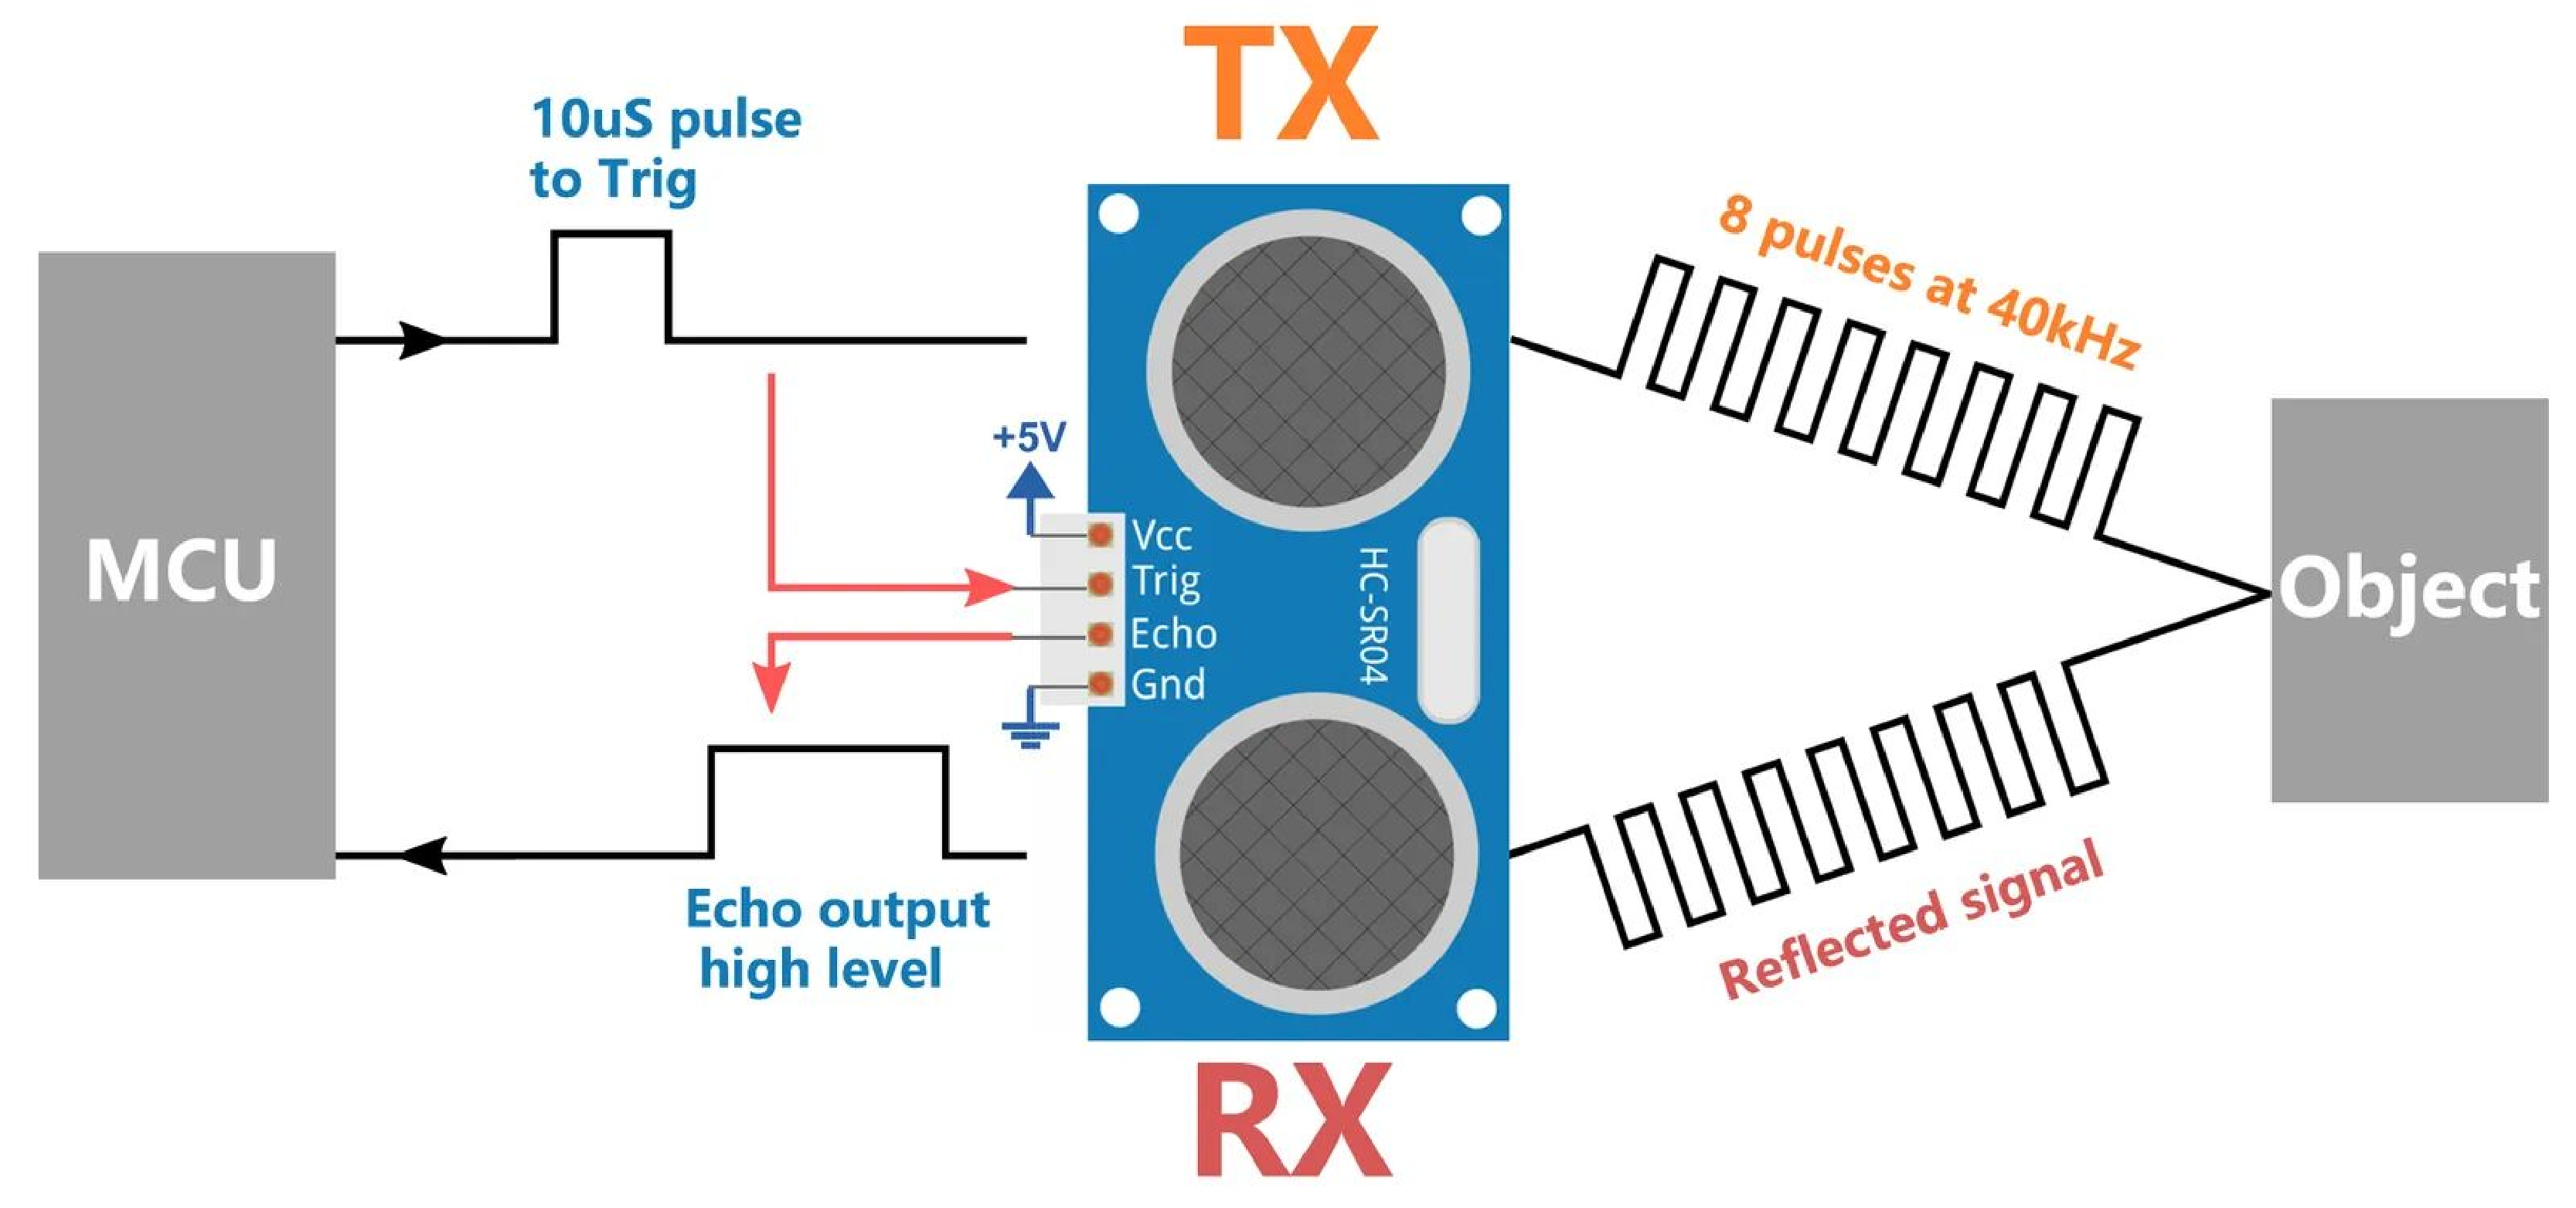
\includegraphics[width=0.8\textwidth]{images/ultrasonic_prin.pdf}
\floatnotes{}
%\label{fig:}
\caption{Ultraschallmodul Prinzip}
\end{figure}

Sensor ist wie ein Fledermaus, die Schallwellen aussendet, um sich zu
orientieren. Wenn du auf einen Knopf drückst (das ist das 10
Mikrosekunden lange Signal), sagst du der >>Fledermaus-Sensor<<, dass
sie ihre >>Ultraschallrufe<< aussenden soll. Diese >>Rufe<< sind sehr,
sehr hoch, viel höher als jedes Geräusch, das wir hören können, und sie
passieren ganz schnell hintereinander, genau 8 Mal in einem winzigen
Moment.

Das ist, als würdest du schnell hintereinander 8 Mal in die Hände
klatschen, nur dass es so schnell und so hoch ist, dass niemand es hören
kann außer der Sensor selbst. Diese speziellen Klatschgeräusche helfen
der >>Fledermaus-Sensor<<, zu erkennen, wie weit Dinge von ihr entfernt
sind, ähnlich wie echte Fledermäuse es tun, wenn sie durch die Nacht
fliegen.

\begin{itemize}
\item
  \textbf{10 Mikrosekunden (10us)}: Der Sensor wird durch ein Signal von
  10 Mikrosekunden (10us) Länge aktiviert, das ist der Startimpuls. Es
  ist wie das Drücken eines Startknopfes, aber es passiert super
  schnell, in nur einem winzigen Bruchteil einer Sekunde.
\item
  \textbf{8-Zyklus-Burst}: sendet einen Ultraschall-Burst, besteht aus 8
  Ultraschallwellen bei einer Frequenz von 40 kHz, um Entfernungen zu
  messen. Stell dir vor, du klatschst 8 Mal ganz schnell hintereinander
  in die Hände -- so ähnlich macht es der Sensor mit Schallwellen, die
  wir aber nicht hören können.
\item
  \textbf{40 kHz (Kilohertz)}: Das ist die Höhe oder Frequenz des
  Ultraschallsignals, das der Sensor aussendet. Kilohertz ist eine
  Einheit, die verwendet wird, um zu beschreiben, wie hoch oder tief ein
  Ton ist. 40 kHz bedeutet, der Ton schwingt 40.000 Mal pro Sekunde. Das
  ist viel höher als das, was das menschliche Ohr hören kann.
\end{itemize}

Das \textbf{menschliche Gehör} kann normalerweise Töne in einem Bereich
von etwa \textbf{20 Hertz (Hz) bis 20.000 Hertz (20 kHz)} wahrnehmen.
Das bedeutet, alles, was unter 20 Hz oder über 20 kHz liegt, können wir
nicht hören. Der Ultraschall, den der Sensor verwendet, liegt also weit
außerhalb des Bereichs, den unsere Ohren erfassen können, weil er bei 40
kHz ist, also doppelt so hoch wie die obere Grenze unseres Hörvermögens.

\hypertarget{berechne-die-entfernung-zu-einem-objekt}{%
\subsubsection{Berechne die Entfernung zu einem
Objekt}\label{berechne-die-entfernung-zu-einem-objekt}}

Angenommen, wir messen die Entfernung zu einem Objekt, das 1 Meter
entfernt ist.

\begin{enumerate}
\def\labelenumi{\arabic{enumi}.}

\item
  \textbf{Trigger-Signal senden}:

  \begin{itemize}
  
  \item
    Der Sensor erhält über den TRIG-Pin ein 10 Mikrosekunden (µs) hohes
    Signal, was ihn veranlasst, einen 8-Zyklus-Burst von
    Ultraschallwellen mit einer Frequenz von 40 kHz zu senden.
  \end{itemize}
\item
  \textbf{Echo-Signal empfangen}:

  \begin{itemize}
  
  \item
    Nach dem Senden des Bursts wartet der Sensor auf das Echo, also das
    Zurückkommen der Ultraschallwellen, nachdem diese vom Objekt
    reflektiert wurden.
  \end{itemize}
\item
  \textbf{Zeitmessung}:

  \begin{itemize}
  
  \item
    Die Zeit vom Senden bis zum Empfangen des Echos wird gemessen.
    Nehmen wir an, die gemessene Zeit (Echo-Zeit) beträgt 5.82
    Millisekunden (ms).
  \end{itemize}
\item
  \textbf{Entfernung berechnen}:

  \begin{itemize}
  
  \item
    Die Entfernung wird mit der Formel berechnet:
  \item
    $\text{Entfernung} = \frac{\text{Zeit des hohen Niveaus} \times \text{Schallgeschwindigkeit}}{2}$
  \item
    Die Schallgeschwindigkeit in Luft beträgt etwa 340 Meter pro Sekunde
    (M/S). Da unsere Zeit in Millisekunden gemessen wurde, müssen wir
    sie in Sekunden umrechnen, um sie in die Formel einzusetzen (1 ms =
    0.001 Sekunden).
  \end{itemize}
\item
  \textbf{Rechnung}:

  \begin{itemize}
  
  \item
    Umrechnung der Echo-Zeit in Sekunden:
    $5.82 \text{ ms} = 0.00582 \text{ s}$.
  \item
    Einsetzen in die Formel:
  \item
    $\text{Entfernung} = \frac{0.00582 \text{ s} \times 340 \text{ m/s}}{2} = \frac{1.9788 \text{ m}}{2} = 0.9894 \text{ m}$
  \end{itemize}
\end{enumerate}

\hypertarget{keywords-ultraschall}{%
\subsubsection{Keywords Ultraschall}\label{keywords-ultraschall}}

\hypertarget{frequenz}{%
\paragraph{Frequenz}\label{frequenz}}

Die Frequenz beschreibt, wie oft eine Schallwelle (oder jede Art von
Welle) in einer Sekunde schwingt. Sie bestimmt die Tonhöhe eines
Geräusches: je höher die Frequenz, desto höher der Ton.

\hypertarget{huxf6rbarkeit}{%
\paragraph{Hörbarkeit}\label{hoerbarkeit}}

Hörbarkeit bezieht sich darauf, ob ein Geräusch in dem Frequenzbereich
liegt, den das menschliche Ohr wahrnehmen kann, typischerweise zwischen
20 Hz und 20.000 Hz (20 kHz).

\hypertarget{schallwellen}{%
\paragraph{Schallwellen}\label{schallwellen}}

Schallwellen sind Schwingungen, die sich durch die Luft oder ein anderes
Medium ausbreiten und von unserem Ohr als Geräusche wahrgenommen werden
können.

\hypertarget{hertz-hz}{%
\paragraph{Hertz (Hz)}\label{hertz-hz}}

Hertz ist die Einheit für Frequenz im Internationalen Einheitensystem
(SI) und beschreibt, wie viele Schwingungen (Zyklen) pro Sekunde
stattfinden.

\hypertarget{huxf6rschwelle}{%
\paragraph{Hörschwelle}\label{hoerschwelle}}

Die Hörschwelle ist die leiseste Lautstärke eines Tons, die gerade noch
gehört werden kann. Sie variiert je nach Frequenz des Tons und von
Person zu Person.

\hypertarget{ultraschall}{%
\paragraph{Ultraschall}\label{ultraschall}}

Ultraschall bezeichnet Schallwellen, die eine höhere Frequenz haben als
der hörbare Bereich für Menschen (über 20 kHz). Sie werden in der
Medizin für bildgebende Verfahren und in anderen Technologien verwendet.

\hypertarget{infraschall}{%
\paragraph{Infraschall}\label{infraschall}}

Infraschall umfasst Frequenzen unterhalb des menschlichen Hörbereichs
(weniger als 20 Hz) und kann von einigen Tieren wahrgenommen werden oder
tritt bei natürlichen Phänomenen wie Erdbeben auf.

\hypertarget{dezibel-db}{%
\paragraph{Dezibel (dB)}\label{dezibel-db}}

Dezibel ist eine Maßeinheit für die Lautstärke (Schalldruckpegel) eines
Geräusches. Sie hilft, die große Spanne an Hörbarkeit menschlichen
Hörens quantitativ zu erfassen.

\hypertarget{schallgeschwindigkeit}{%
\paragraph{Schallgeschwindigkeit}\label{schallgeschwindigkeit}}

Die Schallgeschwindigkeit ist die Geschwindigkeit, mit der sich
Schallwellen durch ein Medium (wie Luft, Wasser oder Stahl) ausbreiten.
In Luft beträgt sie etwa 343 Meter pro Sekunde bei Raumtemperatur.

\hypertarget{echoortung-und-sonar}{%
\paragraph{Echoortung und Sonar}\label{echoortung-und-sonar}}

Echoortung ist die Fähigkeit einiger Tiere (wie Fledermäuse und
Delfine), die Umgebung zu erkunden, indem sie Schall aussenden und das
Echo analysieren. Sonar ist eine technologische Anwendung dieses
Prinzips, das unter Wasser verwendet wird.

\hypertarget{schallisolierung-und-raumakustik}{%
\paragraph{Schallisolierung und
Raumakustik}\label{schallisolierung-und-raumakustik}}

Schallisolierung bezieht sich auf Techniken, um die Übertragung von
Schall von einem Raum zum anderen zu verhindern. Raumakustik beschäftigt
sich mit der Optimierung von Klangqualität und -verteilung in einem
Raum.

\hypertarget{ultraschallbildgebung-sonographie}{%
\paragraph{Ultraschallbildgebung
(Sonographie)}\label{ultraschallbildgebung-sonographie}}

Ultraschallbildgebung ist ein medizinisches Verfahren, das
Ultraschallwellen nutzt, um Bilder vom Inneren des Körpers zu erzeugen,
z.B. um ein ungeborenes Baby im Mutterleib zu sehen.

\hypertarget{schallausbreitung-in-verschiedenen-medien}{%
\paragraph{Schallausbreitung in verschiedenen
Medien}\label{schallausbreitung-in-verschiedenen-medien}}

Schallwellen breiten sich unterschiedlich in verschiedenen Medien (Luft,
Wasser, Festkörper) aus, beeinflusst durch Faktoren wie Dichte und
Elastizität des Mediums.

\hypertarget{frequenzmodulation-und--demodulation}{%
\paragraph{Frequenzmodulation und
-demodulation}\label{frequenzmodulation-und--demodulation}}

Frequenzmodulation (FM) ist eine Technik, bei der die Frequenz einer
Welle geändert wird, um Informationen zu übertragen. Demodulation ist
der umgekehrte Prozess, bei dem die ursprüngliche Information aus der
modulierten Welle zurückgewonnen wird.

\hypertarget{dopplereffekt}{%
\paragraph{Dopplereffekt}\label{dopplereffekt}}

Der Dopplereffekt tritt auf, wenn sich eine Schallquelle relativ zu
einem Beobachter bewegt, was eine wahrgenommene Änderung der Frequenz
des Schalls zur Folge hat (z.B. das An- und Abschwellen des Geräusches
eines vorbeifahrenden Krankenwagens).

\hypertarget{mathematischen-zugang-ultraschall}{%
\subsubsection{Mathematischen Zugang
Ultraschall}\label{mathematischen-zugang-ultraschall}}

\hypertarget{frequenz-f}{%
\paragraph{\texorpdfstring{Frequenz
($f$)}{Frequenz (f)}}\label{frequenz-f}}

\begin{itemize}

\item
  \textbf{Formel}: $f = \frac{1}{T}$, wobei $T$ die Periodendauer
  ist (die Zeit für eine vollständige Schwingung/Zyklus).
\end{itemize}

\hypertarget{huxf6rbarkeit-1}{%
\paragraph{Hörbarkeit}\label{hoerbarkeit-1}}

\begin{itemize}

\item
  Der hörbare Bereich für Menschen liegt zwischen 20 Hz und 20.000 Hz.
  Frequenzen innerhalb dieses Bereichs sind hörbar, Frequenzen außerhalb
  dieses Bereichs sind entweder Ultraschall (\textgreater{} 20 kHz) oder
  Infraschall (\textless{} 20 Hz).
\end{itemize}

\hypertarget{schallwellen-1}{%
\paragraph{Schallwellen}\label{schallwellen-1}}

\begin{itemize}

\item
  \textbf{Geschwindigkeit ($v$) einer Welle}: $v = f \lambda$, wobei
  $\lambda$ die Wellenlänge ist.
\item
  \textbf{Schallgeschwindigkeit in Luft}: etwa 343 m/s bei 20 °C.
\end{itemize}

\hypertarget{hertz-hz-1}{%
\paragraph{Hertz (Hz)}\label{hertz-hz-1}}

\begin{itemize}

\item
  Einheit für Frequenz, 1 Hz = 1 Schwingung pro Sekunde.
\end{itemize}

\hypertarget{huxf6rschwelle-1}{%
\paragraph{Hörschwelle}\label{hoerschwelle-1}}

\begin{itemize}

\item
  Die Hörschwelle variiert je nach Frequenz, wobei etwa 0 dB SPL
  (Schalldruckpegel) für Frequenzen um 1 kHz als leiseste hörbare Töne
  für Menschen gelten.
\end{itemize}

\hypertarget{ultraschall-und-infraschall}{%
\paragraph{Ultraschall und
Infraschall}\label{ultraschall-und-infraschall}}

\begin{itemize}

\item
  \textbf{Ultraschall}: Frequenzen \textgreater{} 20 kHz, nicht hörbar
  für Menschen.
\item
  \textbf{Infraschall}: Frequenzen \textless{} 20 Hz, ebenfalls nicht
  hörbar für Menschen.
\end{itemize}

\hypertarget{dezibel-db-1}{%
\paragraph{Dezibel (dB)}\label{dezibel-db-1}}

\begin{itemize}

\item
  \textbf{Formel zur Berechnung des Schalldruckpegels}:
  $L = 20 \log_{10}(\frac{p}{p_0})$, wobei $p$ der Schalldruck und
  $p_0$ der Referenzschalldruck (üblicherweise 20 µPa in Luft) ist.
\end{itemize}

\hypertarget{schallgeschwindigkeit-1}{%
\paragraph{Schallgeschwindigkeit}\label{schallgeschwindigkeit-1}}

\begin{itemize}

\item
  Abhängig vom Medium. In Luft etwa 343 m/s, in Wasser etwa 1.483 m/s
  und in Stahl etwa 5.960 m/s.
\end{itemize}

\hypertarget{echoortung-und-sonar-1}{%
\paragraph{Echoortung und Sonar}\label{echoortung-und-sonar-1}}

\begin{itemize}

\item
  \textbf{Entfernungsbestimmung}: $D = \frac{1}{2} t v$, wobei $t$
  die Zeit zwischen Aussenden und Empfangen des Echos ist und $v$ die
  Schallgeschwindigkeit im Medium.
\end{itemize}

\hypertarget{frequenzmodulation-und--demodulation-1}{%
\paragraph{Frequenzmodulation und
-demodulation}\label{frequenzmodulation-und--demodulation-1}}

\begin{itemize}

\item
  \textbf{Frequenzmodulation (FM)}:
  $f(t) = f_c + \Delta f \sin(2 \pi f_m t)$, wobei $f_c$ die
  Trägerfrequenz, $\Delta f$ die Frequenzabweichung und $f_m$ die
  Modulationsfrequenz ist.
\end{itemize}

\hypertarget{dopplereffekt-1}{%
\paragraph{Dopplereffekt}\label{dopplereffekt-1}}

\begin{itemize}

\item
  \textbf{Formel für bewegten Beobachter}:
  $f' = f \left(\frac{v \pm v_o}{v \mp v_s}\right)$, wobei $f'$ die
  wahrgenommene Frequenz, $f$ die ursprüngliche Frequenz, $v$ die
  Schallgeschwindigkeit, $v_o$ die Geschwindigkeit des Beobachters und
  $v_s$ die Geschwindigkeit der Quelle ist. Pluszeichen wird
  verwendet, wenn sich Beobachter und Quelle einander nähern,
  Minuszeichen, wenn sie sich voneinander entfernen.
\end{itemize}

\hypertarget{funktionsprinzip-ir-hindernisvermeidungsmodul}{%
\subsection{Funktionsprinzip
IR-Hindernisvermeidungsmodul}\label{funktionsprinzip-ir-hindernisvermeidungsmodul}}

Stell dir vor, das IR-Hindernisvermeidungsmodul ist wie ein Spiel mit
einem Ball, den du wirfst und der zurückkommt, wenn er auf etwas trifft.
Nur dass hier statt einem Ball Infrarotlicht verwendet wird, das wir
nicht sehen können.

\begin{itemize}
\item
  \textbf{IR-Sender-Empfänger-Paar}: Das Modul hat zwei Hauptteile,
  ähnlich wie du zwei Hände hast -- eine zum Werfen des Balls (das ist
  der IR-Sender) und eine zum Fangen (das ist der IR-Empfänger).
\item
  \textbf{Sender emittiert Infrarotlicht}: Der Sender im Modul >>wirft<<
  Infrarotlicht >>Bälle<< aus. Infrarotlicht ist eine Art Licht, das wir
  nicht mit unseren Augen sehen können, aber es ist überall um uns
  herum, zum Beispiel kommt es von der Fernbedienung deines Fernsehers.
\item
  \textbf{Licht trifft auf Hindernisse}: Wenn das Infrarotlicht auf ein
  Hindernis vor dem Modul trifft -- sagen wir, ein Buch auf dem Boden
  oder eine Wand --, wird das Licht von diesem Hindernis
  >>zurückgeworfen<< wie ein Ball, der von einer Wand abprallt.
\item
  \textbf{Empfänger detektiert reflektiertes Licht}: Der IR-Empfänger im
  Modul wartet darauf, das zurückgeworfene Infrarotlicht >>zu fangen<<.
  Wenn er das Licht >>fängt<<, weiß das Modul, dass etwas da ist -- ein
  Hindernis.
\item
  \textbf{Ausgabe eines niedrigen Signals}: Sobald der Empfänger das
  reflektierte Licht erfasst, sagt das Modul: >>Huch, da ist etwas im
  Weg!<< und sendet ein spezielles Signal aus, ein >>niedriges Signal<<,
  um zu zeigen, dass ein Hindernis erkannt wurde. Dieses Signal kann
  dann von einem Computer, einem Roboter oder einem anderen Gerät
  verwendet werden, um zu entscheiden, was als Nächstes zu tun ist, wie
  zum Beispiel anzuhalten oder die Richtung zu ändern.
\end{itemize}

\textbf{Mathematische Annäherung} nutzen, um zu verstehen, wie die
Entfernungsmessung und die Auswirkung der Objektfarbe auf die
Reflexionsniveaus funktionieren. Das Modul verwendet Infrarotlicht, um
Objekte zu erkennen, indem es Licht aussendet und das von Objekten
reflektierte Licht misst. Die Zeit vom Aussenden bis zum Empfang des
reflektierten Lichts gibt Aufschluss über die Entfernung zum Objekt.

\hypertarget{grundlagen-der-entfernungsmessung}{%
\subsubsection{Grundlagen der
Entfernungsmessung}\label{grundlagen-der-entfernungsmessung}}

Die Grundidee hinter der Entfernungsmessung mit einem IR-Sensor basiert
auf der Lichtgeschwindigkeit und der Zeit, die das Licht benötigt, um
zum Sensor zurückzukehren. Für präzise Messungen in kurzen Entfernungen,
wie sie bei IR-Hindernisvermeidungsmodulen üblich sind, berücksichtigt
man die Geschwindigkeit des Lichts und die Verarbeitungszeit des
Sensors.

\hypertarget{einfluss-der-objektfarbe}{%
\paragraph{Einfluss der Objektfarbe}\label{einfluss-der-objektfarbe}}

Die Reflexionseigenschaften von Objekten beeinflussen, wie viel Licht
zum Sensor zurückkehrt. Dunklere Farben absorbieren mehr Licht und
reflektieren weniger, was zu einem schwächeren Signal führt. Helle
Farben reflektieren mehr Licht und führen zu einem stärkeren Signal. Das
Modul misst die Intensität des reflektierten Lichts, um zu bestimmen, ob
ein Objekt innerhalb des Erfassungsbereichs liegt.

\hypertarget{mathematische-betrachtung-der-reflexionsniveaus}{%
\paragraph{Mathematische Betrachtung der
Reflexionsniveaus}\label{mathematische-betrachtung-der-reflexionsniveaus}}

Die Intensität des reflektierten Lichts ($I$) kann durch das
Lambert-Beersche Gesetz angenähert werden, das die Absorption und
Reflexion von Licht durch ein Material beschreibt:

$I = I_0 \, e^{-\alpha d}$

\begin{itemize}

\item
  $I_0$ ist die ursprüngliche Intensität des ausgesendeten Lichts,
\item
  $\alpha$ ist der Absorptionskoeffizient des Materials (höher für
  dunklere Objekte),
\item
  $d$ ist die Dicke des Materials oder die Distanz, die das Licht
  durch das Objekt zurücklegt.
\end{itemize}

Für das IR-Hindernisvermeidungsmodul ist $d$ die Entfernung zum
Objekt, und der Absorptionskoeffizient kann als Maß für die Farbe oder
Reflexionsfähigkeit des Objekts angesehen werden.

\hypertarget{entfernungsberechnung}{%
\paragraph{Entfernungsberechnung}\label{entfernungsberechnung}}

Angenommen, ein IR-Sensor misst die Zeit $t = 1 \times 10^{-4}$
Sekunden für das Licht, um von einem Objekt reflektiert zu werden und
zurückzukehren. Die Entfernung ($d$) zum Objekt kann berechnet werden
als:

$d = \frac{c \cdot t}{2}$

Wobei $c$ die Lichtgeschwindigkeit ist. Für kurze Distanzen und die
schnelle Reflexion von Infrarotlicht ist jedoch die genaue
Geschwindigkeit des Lichts oft weniger relevant als die direkte Messung
der Zeit und die Kalibrierung des Sensors.

Infrarot-Hindernisvermeidungsmodule nutzen die Prinzipien der
Lichtreflexion und -absorption, um Objekte innerhalb eines bestimmten
Bereichs zu erkennen. Die Farbe des Objekts beeinflusst die
Reflexionsniveaus, und die Sensorik ist darauf ausgelegt, diese
Unterschiede zu erfassen und zu interpretieren, um Hindernisse zu
identifizieren. Die mathematische Modellierung dieser Prozesse
ermöglicht ein tieferes Verständnis ihrer Funktionsweise und der
Faktoren, die die Sensorleistung beeinflussen.

\hypertarget{effektive-winkel-von-35}{%
\subsubsection{effektive Winkel von 35°}\label{effektive-winkel-von-35}}

Der \textbf{effektive Winkel von 35°} bei einem
IR-Hindernisvermeidungsmodul bezieht sich auf den Winkelbereich,
innerhalb dessen das Modul effektiv Hindernisse erkennen kann.

\begin{itemize}
\item
  \textbf{Fokussierte Erkennung}: Der Sensor kann Objekte innerhalb
  eines Kegels erkennen, der im Zentrum eine Spitze hat (dort, wo der
  Sensor montiert ist) und sich mit einem Öffnungswinkel von 35° nach
  außen ausweitet. Dies begrenzt die Erkennungszone auf einen
  spezifischen Bereich vor dem Sensor.
\item
  \textbf{Planung der Sensorplatzierung}: Für eine umfassende Abdeckung
  rund um den Roboter könnten mehrere Sensoren benötigt werden, da jeder
  Sensor nur Hindernisse innerhalb seines effektiven Winkels von 35°
  erkennen kann. Durch strategische Platzierung dieser Sensoren kann ein
  Roboter eine 360°-Hinderniserkennung erreichen.
\item
  \textbf{Navigationsgenauigkeit}: Der effektive Winkel beeinflusst, wie
  genau der Roboter seine Umgebung >>sieht<<. Ein schmalerer Winkel
  bietet eine genauere Erkennung in die Tiefe des Feldes, während ein
  breiterer Winkel eine breitere, aber weniger präzise Erkennung
  ermöglicht. Mit 35° bietet der Sensor eine ausgewogene Mischung aus
  Breite und Genauigkeit.
\item
  \textbf{Vermeidungsstrategien}: Der Roboter verwendet die
  Informationen aus dem Sensor, um Kollisionen zu vermeiden. Mit einem
  effektiven Winkel von 35° muss der Roboter möglicherweise seine Route
  anpassen, wenn ein Hindernis innerhalb dieses Bereichs erkannt wird,
  was die Bewegungsplanung und Strategie zur Hindernisvermeidung
  beeinflusst.
\end{itemize}

Die Montage der IR-Hindernisvermeidungsmodul in einem Winkel von 35°
nach vorne außen, zusammen mit einem zentralen Ultraschallsensor, eine
kluge Wahl für die Optimierung der Hinderniserkennung und -vermeidung
bei einem Rover ist. Diese Anordnung erhöht die räumliche Wahrnehmung
und ermöglicht eine effektivere Navigation in komplexen Umgebungen.

\hypertarget{keywords-infrarotlicht-ir}{%
\subsubsection{Keywords Infrarotlicht
(IR)}\label{keywords-infrarotlicht-ir}}

\begin{enumerate}
\def\labelenumi{\arabic{enumi}.}
\item
  \textbf{Wellenlänge}: Der Abstand zwischen zwei aufeinanderfolgenden
  Wellenbergen oder -tälern in einer Welle. Bestimmt Farbe und Energie
  des Lichts.
\item
  \textbf{Sichtbares Licht}: Der Teil des elektromagnetischen Spektrums,
  den das menschliche Auge sehen kann, von Violett bis Rot.
\item
  \textbf{Elektromagnetisches Spektrum}: Die gesamte Bandbreite
  elektromagnetischer Wellen, von sehr kurzen Gammastrahlen bis zu sehr
  langen Radiowellen, einschließlich sichtbarem Licht.
\item
  \textbf{Infrarotlicht (IR)}: Lichtwellen, die länger als rotes Licht
  sind und von uns als Wärme gefühlt, aber nicht gesehen werden können.
\item
  \textbf{Ultraviolettes Licht (UV)}: Lichtwellen, die kürzer als
  violettes Licht sind und Hautbräunung oder -schäden verursachen
  können.
\item
  \textbf{Nanometer (nm)}: Eine Einheit zur Messung der Wellenlänge des
  Lichts, wobei 1 Nanometer einem milliardsten Meter entspricht.
\item
  \textbf{Photonen}: Teilchen, die Lichtwellen tragen. Sie sind die
  kleinsten Energiequanten im Licht.
\item
  \textbf{Farbspektrum}: Die Reihe von Farben, die durch das Aufteilen
  von Licht in seine einzelnen Wellenlängen entsteht, z.B. durch ein
  Prisma.
\item
  \textbf{Transparenz und Opazität}: Eigenschaften von Materialien, die
  bestimmen, ob Licht durch sie hindurchgehen kann (transparent) oder
  nicht (opak).
\item
  \textbf{Reflexion und Brechung}: Reflexion ist das Zurückwerfen von
  Licht von einer Oberfläche. Brechung ist die Änderung der Richtung des
  Lichts, wenn es von einem Medium in ein anderes übergeht.
\item
  \textbf{Lichtabsorption}: Wenn Materialien Licht aufnehmen und in eine
  andere Energieform umwandeln, oft Wärme.
\item
  \textbf{Prisma und Lichtdispersion}: Ein Prisma kann Licht in sein
  Farbspektrum aufteilen, indem es die verschiedenen Wellenlängen
  unterschiedlich bricht.
\item
  \textbf{Nachtsicht und Infrarottechnologien}: Technologien, die
  Infrarotlicht nutzen, um in der Dunkelheit zu sehen oder Bilder zu
  erzeugen.
\item
  \textbf{Wärmebildtechnik}: Eine Technik, die Temperaturunterschiede in
  einer Szene erfasst und sie in ein sichtbares Bild umwandelt,
  basierend auf Infrarotstrahlung.
\item
  \textbf{Lichtquellen}: Objekte oder Geräte, die Licht aussenden, wie
  die Sonne, Glühbirnen oder Laser.
\item
  \textbf{Farbtemperatur}: Ein Maß für die Lichtfarbe, gemessen in
  Kelvin (K), das angibt, ob das Licht eher warm (gelblich) oder kühl
  (bläulich) ist.
\item
  \textbf{Lasertechnologie}: Technologie, die Licht durch einen Prozess
  der optischen Verstärkung erzeugt, was zu einem sehr engen und
  fokussierten Lichtstrahl führt.
\item
  \textbf{Holographie}: Eine Technik zur Erzeugung dreidimensionaler
  Bilder mit Laserlicht.
\item
  \textbf{Elektromagnetische Wellentheorie}: Die Theorie, die die
  Ausbreitung elektromagnetischer Wellen, einschließlich Licht, durch
  Raum oder Materie beschreibt.
\end{enumerate}

\hypertarget{mathematischen-zugang-infrarotlicht-ir}{%
\subsubsection{Mathematischen Zugang Infrarotlicht
(IR)}\label{mathematischen-zugang-infrarotlicht-ir}}

\hypertarget{wellenluxe4nge-lambda}{%
\paragraph{\texorpdfstring{1. Wellenlänge
($\lambda$)}{1. Wellenlänge (\textbackslash lambda)}}\label{wellenlaenge-lambda}}

\begin{itemize}

\item
  \textbf{Mathematische Darstellung}: $\lambda = \frac{v}{f}$

  \begin{itemize}
  
  \item
    $v$ ist die Geschwindigkeit der Welle (z.B. Lichtgeschwindigkeit
    im Vakuum, etwa $3 \times 10^8$ m/s).
  \item
    $f$ ist die Frequenz der Welle in Hertz (Hz).
  \end{itemize}
\end{itemize}

\hypertarget{sichtbares-licht-und-elektromagnetisches-spektrum}{%
\paragraph{2. Sichtbares Licht und Elektromagnetisches
Spektrum}\label{sichtbares-licht-und-elektromagnetisches-spektrum}}

\begin{itemize}

\item
  \textbf{Bereich des sichtbaren Lichts}: Etwa 380 nm bis 740 nm.
\item
  \textbf{Umrechnung in Frequenz}: $f = \frac{c}{\lambda}$, wobei
  $c$ die Lichtgeschwindigkeit ist.
\end{itemize}

\hypertarget{infrarotlicht-ir-und-ultraviolettes-licht-uv}{%
\paragraph{3. Infrarotlicht (IR) und Ultraviolettes Licht
(UV)}\label{infrarotlicht-ir-und-ultraviolettes-licht-uv}}

\begin{itemize}

\item
  \textbf{IR-Bereich}: Wellenlängen größer als 740 nm.
\item
  \textbf{UV-Bereich}: Wellenlängen kleiner als 380 nm.
\item
  \textbf{Berechnung der Energie eines Photons}:
  $E = hf = \frac{hc}{\lambda}$, wobei $h$ das Plancksche
  Wirkungsquantum ist.
\end{itemize}

\hypertarget{nanometer-nm}{%
\paragraph{4. Nanometer (nm)}\label{nanometer-nm}}

\begin{itemize}

\item
  \textbf{Umrechnung}: 1 nm = $10^{-9}$ Meter.
\item
  \textbf{Anwendung in Formeln}: Direkte Einsetzung der Wellenlänge in
  nm nach Umrechnung in Meter für physikalische Berechnungen.
\end{itemize}

\hypertarget{transparenz-reflexion-brechung-und-lichtabsorption}{%
\paragraph{5. Transparenz, Reflexion, Brechung, und
Lichtabsorption}\label{transparenz-reflexion-brechung-und-lichtabsorption}}

\begin{itemize}

\item
  \textbf{Brechungsindex}: $n = \frac{c}{v_{medium}}$, wobei
  $v_{medium}$ die Geschwindigkeit des Lichts im Medium ist.
\item
  \textbf{Snelliussches Brechungsgesetz}:
  $n_1 \sin(\theta_1) = n_2 \sin(\theta_2)$, wobei $\theta$ der
  Winkel zur Normalen ist.
\end{itemize}

\hypertarget{prisma-und-lichtdispersion}{%
\paragraph{6. Prisma und
Lichtdispersion}\label{prisma-und-lichtdispersion}}

\begin{itemize}

\item
  \textbf{Dispersion}: Abhängigkeit des Brechungsindex von der
  Wellenlänge, was zu Farbaufspaltung führt.
\end{itemize}

\hypertarget{farbtemperatur}{%
\paragraph{7. Farbtemperatur}\label{farbtemperatur}}

\begin{itemize}

\item
  \textbf{Einheit}: Kelvin (K).
\item
  \textbf{Zusammenhang mit Spektrum}: Höhere Farbtemperaturen
  entsprechen bläulicherem Licht, niedrigere wärmerem Licht.
\end{itemize}

\hypertarget{lasertechnologie-und-holographie}{%
\paragraph{8. Lasertechnologie und
Holographie}\label{lasertechnologie-und-holographie}}

\begin{itemize}

\item
  \textbf{Kohärenz und Monochromasie}: Laserlicht hat sehr enge
  Wellenlängenbereiche, ideal für Interferenz und Holographie.
\end{itemize}

\hypertarget{photonik-und-elektromagnetische-wellentheorie}{%
\paragraph{9. Photonik und Elektromagnetische
Wellentheorie}\label{photonik-und-elektromagnetische-wellentheorie}}

\begin{itemize}

\item
  \textbf{Photonenenergie}: Siehe Formel oben.
\item
  \textbf{Maxwellsche Gleichungen}: Grundlage der elektromagnetischen
  Wellentheorie, beschreiben die Ausbreitung elektromagnetischer Felder.
\end{itemize}

\hypertarget{funktionsprinzip-servo}{%
\subsection{Funktionsprinzip Servo}\label{funktionsprinzip-servo}}

\hypertarget{motor}{%
\paragraph{Motor}\label{motor}}

\begin{itemize}

\item
  Im Servo befindet sich ein Motor, ähnlich denen, die die Räder eines
  Marsrovers antreiben könnten. Dieser Motor ist für die Bewegung
  zuständig.
\end{itemize}

\hypertarget{die-kraft-der-uxfcbersetzung-zahnruxe4der}{%
\paragraph{Die Kraft der Übersetzung:
Zahnräder}\label{die-kraft-der-uebersetzung-zahnraeder}}

\begin{itemize}

\item
  Um die Motorbewegung zu kontrollieren und kraftvoller zu machen, sind
  um den Motor herum Zahnräder angeordnet. Ein großes Zahnrad greift in
  ein kleineres ein, das direkt auf der Motorwelle sitzt. Diese
  Anordnung wandelt die schnelle Drehung des Motors in eine langsamere,
  aber stärkere Bewegung um. Das ist wichtig, weil wir oft wollen, dass
  der Rover präzise und kraftvoll agiert, zum Beispiel beim Bewegen
  seiner Arme oder beim Drehen seines Körpers.
\end{itemize}

\hypertarget{potentiometer-und-steuerungsschaltung}{%
\paragraph{Potentiometer und
Steuerungsschaltung}\label{potentiometer-und-steuerungsschaltung}}

\begin{itemize}

\item
  Ein wichtiger Teil des Servos ist das Potentiometer. Stell dir das
  Potentiometer wie einen kleinen Detektiv vor, der immer genau weiß, in
  welcher Position sich der Servo befindet. Wenn sich der Servo dreht,
  dreht sich auch das Potentiometer und verändert seinen Widerstand.
\item
  Die Steuerungsschaltung im Servo ist wie das Gehirn, das die
  Informationen des Potentiometers liest. Sie versteht die Veränderung
  des Widerstands und weiß dadurch, in welcher Position sich der Servo
  befindet. So kann sie den Servo genau dort anhalten, wo er sein soll.
\end{itemize}

\hypertarget{pulsweitenmodulation-pwm}{%
\paragraph{Pulsweitenmodulation (PWM)}\label{pulsweitenmodulation-pwm}}

\begin{itemize}

\item
  Durch die Anpassung der >>Länge<< (also der Impulse) können wir den
  Servo sehr genau steuern. So können wir dem Rover befehlen, seinen Arm
  genau so zu bewegen, wie wir es möchten, oder sich in eine bestimmte
  Richtung zu drehen.
\end{itemize}

\hypertarget{newton}{%
\subsection{Newton}\label{newton}}

Ein \textbf{Newton} (Symbol: \textbf{N}) ist die SI-Einheit der Kraft.
Sie ist definiert als die Kraft, die erforderlich ist, um einem
Kilogramm Masse eine Beschleunigung von einem Meter pro Sekunde im
Quadrat zu erteilen. Mathematisch ausgedrückt:

$1 \, \text{N} = 1 \, \text{kg} \cdot \text{m} / \text{s}^2$

Das bedeutet, dass ein Newton die Menge an Kraft ist, die benötigt wird,
um ein Objekt mit einer Masse von einem Kilogramm mit einer Rate von
einem Meter pro Sekunde pro Sekunde zu beschleunigen.

\hypertarget{mathematischer-zugang-zu-newton}{%
\subsubsection{Mathematischer Zugang zu
Newton}\label{mathematischer-zugang-zu-newton}}

Die Beziehung zwischen den Grundgrößen in der Physik, wie Masse,
Beschleunigung und Kraft, kann durch das zweite Newtonsche Gesetz
ausgedrückt werden:

$F = m \cdot a$

\begin{itemize}

\item
  $F$ ist die Kraft in Newton,
\item
  $m$ ist die Masse in Kilogramm,
\item
  $a$ ist die Beschleunigung in Metern pro Sekunde im Quadrat
  ($m/s^2$).
\end{itemize}

\hypertarget{rechenbeispiel-kraftberechnung}{%
\paragraph{Rechenbeispiel:
Kraftberechnung}\label{rechenbeispiel-kraftberechnung}}

Angenommen, ein Auto mit einer Masse von 1000 kg soll aus dem Stand
innerhalb von 5 Sekunden auf eine Geschwindigkeit von 10 m/s
beschleunigt werden. Die Beschleunigung ($a$) kann zuerst berechnet
werden als:

$a = \frac{\Delta v}{\Delta t} = \frac{10 \, \text{m/s}}{5 \, \text{s}} = 2 \, \text{m/s}^2$

Dann kann die Kraft ($F$) berechnet werden, die benötigt wird, um
diese Beschleunigung zu erreichen:

$F = m \cdot a = 1000 \, \text{kg} \cdot 2 \, \text{m/s}^2 = 2000 \, \text{N}$

Das bedeutet, dass eine Kraft von 2000 Newton erforderlich ist, um das
Auto unter den gegebenen Bedingungen zu beschleunigen.

\hypertarget{unterschied-zwischen-gewicht-und-masse}{%
\subsubsection{Unterschied zwischen Gewicht und
Masse}\label{unterschied-zwischen-gewicht-und-masse}}

\begin{itemize}

\item
  \textbf{Masse}: Ein Maß für die Menge an Materie in einem Objekt. Die
  Masse ist eine inhärente Eigenschaft eines Objekts und ändert sich
  nicht, unabhängig von der Position im Universum.
\item
  \textbf{Gewicht}: Eine Kraft, die aufgrund der Gravitationsanziehung
  auf eine Masse wirkt. Das Gewicht kann variieren, abhängig von der
  Gravitationsbeschleunigung des Ortes, an dem sich das Objekt befindet.
\end{itemize}

\hypertarget{umrechnung-zwischen-kilogramm-und-newton}{%
\paragraph{Umrechnung zwischen Kilogramm und
Newton}\label{umrechnung-zwischen-kilogramm-und-newton}}

Die Umrechnung zwischen Kilogramm (kg) und Newton (N) hängt von der
Gravitationsbeschleunigung ab. Auf der Erdoberfläche beträgt die
durchschnittliche Gravitationsbeschleunigung etwa
$9,81 \, \text{m/s}^2$.

$1 \, \text{kg} \approx 9,81 \, \text{N}$

Das bedeutet, dass die Gewichtskraft eines Körpers mit der Masse 1 kg
auf der Erdoberfläche etwa 9,81 N beträgt.

\hypertarget{was-ist-gravitationsbeschleunigung}{%
\subsubsection{Was ist
Gravitationsbeschleunigung?}\label{was-ist-gravitationsbeschleunigung}}

Stell dir vor, du lässt einen Ball fallen. Während der Ball fällt, wird
er schneller und schneller. Das liegt daran, dass die Erde eine Art
unsichtbare Kraft hat, die alles zu sich zieht -- wir nennen das
Gravitation. Die Gravitationsbeschleunigung ist ein Maß dafür, wie
schnell etwas durch diese Kraft beschleunigt wird, wenn es fällt.

Die Zahl $9,81 \, \text{m/s}^2$ sagt uns, wie schnell der Ball jedes
Sekunde schneller wird, wenn er fällt. Das bedeutet, am Ende der ersten
Sekunde fällt der Ball mit einer Geschwindigkeit von
$9,81 \, \text{Meter pro Sekunde}$. Nach zwei Sekunden ist er schon
doppelt so schnell, also etwa $19,62 \, \text{Meter pro Sekunde}$, und
so wird er immer schneller, je länger er fällt.

\hypertarget{experiment-freier-fall---volle-und-eine-leere-flasche-gleichzeitig-fallen}{%
\paragraph{Experiment freier Fall - volle und eine leere Flasche
gleichzeitig
fallen}\label{experiment-freier-fall---volle-und-eine-leere-flasche-gleichzeitig-fallen}}

Wenn du eine volle und eine leere Flasche gleichzeitig fallen lässt,
fallen sie tatsächlich mit der gleichen Geschwindigkeit, vorausgesetzt,
dass sie im Vakuum fallen, wo kein Luftwiderstand vorhanden ist. Das
liegt daran, dass die Gravitationsbeschleunigung für alle Objekte an
einem bestimmten Ort gleich ist, unabhängig von ihrer Masse. Dieses
Prinzip wurde von Galileo Galilei durch seine Experimente im 16.
Jahrhundert entdeckt und später von Isaac Newton in seinen
Bewegungsgesetzen formuliert.

In der realen Welt, außerhalb eines Vakuums, spielt jedoch der
Luftwiderstand eine Rolle. Der Luftwiderstand hängt von verschiedenen
Faktoren ab, einschließlich der Form des Objekts und seiner Oberfläche.
Wenn die volle und die leere Flasche genau dieselbe Form und Größe
haben, könnte die volle Flasche schneller fallen als die leere, weil sie
eine größere Masse hat und der Unterschied im Luftwiderstand zwischen
beiden Flaschen nicht ausreicht, um den Fall der schwereren Flasche
signifikant zu verlangsamen. Aber der Unterschied wäre unter normalen
Bedingungen minimal.

In der Praxis bedeutet das, dass, obwohl theoretisch beide Flaschen mit
der gleichen Rate fallen sollten, die volle Flasche aufgrund ihres
größeren Gewichts leicht schneller fallen könnte als die leere Flasche,
besonders wenn die Flaschen nicht perfekt aerodynamisch sind und der
Luftwiderstand eine Rolle spielt.

\hypertarget{keywords-gravitation-newtonsche-gesetze-und-die-grundlegenden-physikalischen-einheiten}{%
\subsubsection{Keywords Gravitation, Newtonsche Gesetze und die
grundlegenden physikalischen
Einheiten}\label{keywords-gravitation-newtonsche-gesetze-und-die-grundlegenden-physikalischen-einheiten}}

\begin{enumerate}
\def\labelenumi{\arabic{enumi}.}

\item
  \textbf{Gravitation}: Anziehungskraft zwischen Massen,
  Gravitationsfeld, Gravitationsgesetz, universelle
  Gravitationskonstante.
\item
  \textbf{Newton}: Isaac Newton, Newtonsche Gesetze der Bewegung,
  Newtonsches Gravitationsgesetz, Einheit der Kraft.
\item
  \textbf{Kraft}: Grundlegende Wechselwirkung, Newton (N), Kraftvektor,
  resultierende Kraft, Zentripetalkraft.
\item
  \textbf{Beschleunigung}: Änderungsrate der Geschwindigkeit, $m/s^2$,
  gleichmäßige Beschleunigung, Gravitationsbeschleunigung.
\item
  \textbf{Masse}: Menge der Materie, Kilogramm (kg), Trägheit,
  Massenerhaltung.
\item
  \textbf{Gewicht}: Kraft aufgrund der Gravitation, Gewichtskraft,
  Unterschied zwischen Masse und Gewicht, $N$ (Newton).
\item
  \textbf{Meter (m)}: Basiseinheit der Länge, Distanzmessung,
  Lichtgeschwindigkeit in Metern pro Sekunde.
\item
  \textbf{Kilogramm (kg)}: Basiseinheit der Masse, internationaler
  Kilogrammprototyp, Masse-Wasser-Äquivalent.
\item
  \textbf{Sekunde (s)}: Basiseinheit der Zeit, Zeitmessung, Frequenz des
  Cäsium-133-Atoms.
\item
  \textbf{Ampere (A)}: Basiseinheit der elektrischen Stromstärke,
  elektrischer Strom, Coulombs pro Sekunde.
\item
  \textbf{Kelvin (K)}: Basiseinheit der Temperatur, absolute
  Temperaturskala, thermodynamische Temperatur.
\item
  \textbf{Mol (mol)}: Basiseinheit der Stoffmenge, Avogadros Zahl,
  Moleküle und Atome.
\item
  \textbf{Candela (cd)}: Basiseinheit der Lichtstärke, Lichtquellen,
  Luminanz.
\item
  \textbf{Fallgesetze}: Freier Fall, Luftwiderstand,
  Terminalgeschwindigkeit.
\item
  \textbf{Impuls und Impulserhaltung}: Impuls als Produkt aus Masse und
  Geschwindigkeit, Erhaltungsgesetz.
\item
  \textbf{Arbeit und Energie}: Arbeitseinheit Joule, kinetische Energie,
  potenzielle Energie, Energieerhaltung.
\item
  \textbf{Drehmoment}: Rotationskraft, Drehmoment und Hebelgesetz,
  $N\cdot m$ (Newtonmeter).
\item
  \textbf{Schwingungen und Wellen}: Periodische Bewegung, Frequenz,
  Wellenlänge, Schallwellen, elektromagnetische Wellen.
\end{enumerate}

\hypertarget{mathematischen-zugang-gravitation-newtonsche-gesetze-und-die-grundlegenden-physikalischen-einheiten}{%
\subsubsection{Mathematischen Zugang Gravitation, Newtonsche Gesetze und
die grundlegenden physikalischen
Einheiten}\label{mathematischen-zugang-gravitation-newtonsche-gesetze-und-die-grundlegenden-physikalischen-einheiten}}

\hypertarget{gravitation}{%
\paragraph{Gravitation}\label{gravitation}}

\begin{itemize}

\item
  \textbf{Newtonsches Gravitationsgesetz}: $F = G \frac{m_1 m_2}{r^2}$

  \begin{itemize}
  
  \item
    \textbf{Beispiel}: Zwei Massen von je 1 kg im Abstand von 1 m
    zueinander üben eine Anziehungskraft von etwa
    $6,674 \times 10^{-11} \, \text{N}$ aus.
  \end{itemize}
\end{itemize}

\hypertarget{newton-1}{%
\paragraph{Newton}\label{newton-1}}

\begin{itemize}

\item
  \textbf{Zweites Newtonsches Gesetz}: $F = m \cdot a$

  \begin{itemize}
  
  \item
    \textbf{Beispiel}: Ein Objekt mit einer Masse von 10 kg, das mit
    $2 \, \text{m/s}^2$ beschleunigt wird, erfährt eine Kraft von
    $20 \, \text{N}$.
  \end{itemize}
\end{itemize}

\hypertarget{kraft}{%
\paragraph{Kraft}\label{kraft}}

\begin{itemize}

\item
  \textbf{Kraftvektor}: $F = m \cdot a$

  \begin{itemize}
  
  \item
    \textbf{Beispiel}: Ein Auto (Masse = 1000 kg) beschleunigt mit
    $1 \, \text{m/s}^2$, die wirkende Kraft ist $1000 \, \text{N}$.
  \end{itemize}
\end{itemize}

\hypertarget{beschleunigung}{%
\paragraph{Beschleunigung}\label{beschleunigung}}

\begin{itemize}

\item
  \textbf{Gleichmäßige Beschleunigung}:
  $a = \frac{\Delta v}{\Delta t}$

  \begin{itemize}
  
  \item
    \textbf{Beispiel}: Ein Auto erhöht seine Geschwindigkeit von 0 auf
    $60 \, \text{km/h}$ (etwa $16,67 \, \text{m/s}$) in 5 Sekunden,
    $a = 3,33 \, \text{m/s}^2$.
  \end{itemize}
\end{itemize}

\hypertarget{masse-und-gewicht}{%
\paragraph{Masse und Gewicht}\label{masse-und-gewicht}}

\begin{itemize}

\item
  \textbf{Gewicht}: $W = m \cdot g$

  \begin{itemize}
  
  \item
    \textbf{Beispiel}: Eine Masse von 50 kg auf der Erde (mit
    $g = 9,81 \, \text{m/s}^2$) hat ein Gewicht von
    $490,5 \, \text{N}$.
  \end{itemize}
\end{itemize}

\hypertarget{meter-und-kilogramm}{%
\paragraph{Meter und Kilogramm}\label{meter-und-kilogramm}}

\begin{itemize}

\item
  \textbf{Längenmessung}: 1 Meter ist die Basislänge.
\item
  \textbf{Masse}: 1 Kilogramm ist die Basismasse.
\end{itemize}

\hypertarget{sekunde-ampere-kelvin-mol-candela}{%
\paragraph{Sekunde, Ampere, Kelvin, Mol,
Candela}\label{sekunde-ampere-kelvin-mol-candela}}

\begin{itemize}

\item
  \textbf{Zeit}: 1 Sekunde ist die Basiseinheit der Zeit.
\item
  \textbf{Stromstärke}: 1 Ampere ist die Basiseinheit der elektrischen
  Stromstärke.
\item
  \textbf{Temperatur}: 1 Kelvin ist die Basiseinheit der Temperatur.
\item
  \textbf{Stoffmenge}: 1 Mol ist die Basiseinheit der Stoffmenge.
\item
  \textbf{Lichtstärke}: 1 Candela ist die Basiseinheit der Lichtstärke.
\end{itemize}

\hypertarget{fallgesetze-und-impulserhaltung}{%
\paragraph{Fallgesetze und
Impulserhaltung}\label{fallgesetze-und-impulserhaltung}}

\begin{itemize}

\item
  \textbf{Freier Fall}: $s = \frac{1}{2} g t^2$

  \begin{itemize}
  
  \item
    \textbf{Beispiel}: Ein Objekt fällt für 2 Sekunden, zurückgelegte
    Strecke ist $19,62 \, \text{m}$.
  \end{itemize}
\end{itemize}

\hypertarget{arbeit-und-energie}{%
\paragraph{Arbeit und Energie}\label{arbeit-und-energie}}

\begin{itemize}

\item
  \textbf{Arbeit}: $W = F \cdot d$

  \begin{itemize}
  
  \item
    \textbf{Beispiel}: Heben eines Objekts (Kraft = 100 N) um 2 Meter
    verrichtet eine Arbeit von $200 \, \text{J}$.
  \end{itemize}
\end{itemize}

\hypertarget{drehmoment}{%
\paragraph{Drehmoment}\label{drehmoment}}

\begin{itemize}

\item
  \textbf{Drehmoment}: $\tau = F \cdot r$

  \begin{itemize}
  
  \item
    \textbf{Beispiel}: Eine Kraft von $10 \, \text{N}$, die im Abstand
    von 0,5 m vom Drehpunkt wirkt, erzeugt ein Drehmoment von
    $5 \, \text{N}\cdot\text{m}$.
  \end{itemize}
\end{itemize}

\hypertarget{schwingungen-und-wellen}{%
\paragraph{Schwingungen und Wellen}\label{schwingungen-und-wellen}}

\begin{itemize}

\item
  \textbf{Frequenz einer Welle}: $f = \frac{1}{T}$

  \begin{itemize}
  
  \item
    \textbf{Beispiel}: Eine Schwingung, die sich alle 0,5 Sekunden
    wiederholt, hat eine Frequenz von $2 \, \text{Hz}$.
  \end{itemize}
\end{itemize}

\hypertarget{gravitationsbeschleunigungen-fuxfcr-erde-mond-und-mars}{%
\subsubsection{Gravitationsbeschleunigungen für Erde, Mond und
Mars}\label{gravitationsbeschleunigungen-fuer-erde-mond-und-mars}}

Die Gravitationsbeschleunigung eines Himmelskörpers hängt hauptsächlich
von zwei Faktoren ab:

\begin{enumerate}
\def\labelenumi{\arabic{enumi}.}
\item
  \textbf{Masse des Himmelskörpers}: Je größer die Masse eines
  Himmelskörpers ist, desto stärker ist seine Gravitationskraft. Nach
  dem Gravitationsgesetz von Newton ist die Gravitationskraft direkt
  proportional zur Masse des Himmelskörpers. Das bedeutet, dass ein
  Planet mit einer höheren Masse eine stärkere Gravitationsanziehung
  hat, was zu einer höheren Gravitationsbeschleunigung führt.
\item
  \textbf{Radius des Himmelskörpers}: Die Gravitationsbeschleunigung
  hängt auch invers quadratisch vom Radius des Himmelskörpers ab. Wenn
  man sich weiter vom Zentrum eines Himmelskörpers entfernt, nimmt die
  Gravitationsbeschleunigung ab. Dies bedeutet, dass bei zwei
  Himmelskörpern mit gleicher Masse der Körper mit dem kleineren Radius
  eine höhere Gravitationsbeschleunigung an seiner Oberfläche haben
  wird, da man näher am Massenzentrum ist.
\end{enumerate}

Mathematisch wird die Gravitationsbeschleunigung ($g$) an der
Oberfläche eines Himmelskörpers durch die Formel

$g = \frac{G \cdot M}{R^2}$

ausgedrückt, wobei:

\begin{itemize}

\item
  $G$ die universelle Gravitationskonstante ist
  ($6,674 \times 10^{-11} \, \text{m}^3 \text{kg}^{-1} \text{s}^{-2}$),
\item
  $M$ die Masse des Himmelskörpers ist,
\item
  $R$ der Radius des Himmelskörpers ist.
\end{itemize}

\begin{lstlisting}[language=Python]
# Gegebene Werte für Erde, Mond und Mars
# Universelle Gravitationskonstante
G = 6.674 * 10**-11  # m^3 kg^-1 s^-2

# Erde
M_Erde = 5.972 * 10**24  # kg
R_Erde = 6.371 * 10**6  # m

# Mond
M_Mond = 7.347 * 10**22  # kg
R_Mond = 1.737 * 10**6  # m

# Mars
M_Mars = 6.417 * 10**23  # kg
R_Mars = 3.3895 * 10**6  # m

# Berechnung der Gravitationsbeschleunigung für Erde, Mond und Mars
g_Erde = (G * M_Erde) / (R_Erde**2)
g_Mond = (G * M_Mond) / (R_Mond**2)
g_Mars = (G * M_Mars) / (R_Mars**2)

# Ausgabe der Gravitationsbeschleunigungen für Erde, Mond und Mars
print("Gravitationsbeschleunigung auf der Erde:", g_Erde, "m/s^2")
print("Gravitationsbeschleunigung auf dem Mond:", g_Mond, "m/s^2")
print("Gravitationsbeschleunigung auf dem Mars:", g_Mars, "m/s^2")
\end{lstlisting}

Die Gravitationsbeschleunigung eines Himmelskörpers hat signifikante
Auswirkungen auf unseren Körper, vor allem in Bezug auf unser Gewicht,
unsere Muskulatur und das Skelettsystem.

\hypertarget{gewichtsunterschiede}{%
\subsubsection{Gewichtsunterschiede}\label{gewichtsunterschiede}}

\begin{itemize}

\item
  \textbf{Erde}: Auf der Erde erfahren wir die
  Gravitationsbeschleunigung, die unser Körper gewohnt ist. Unser
  Gewicht auf der Erde dient als Referenzwert für Vergleiche mit anderen
  Himmelskörpern.
\item
  \textbf{Mond}: Auf dem Mond beträgt die Gravitationsbeschleunigung nur
  etwa 1/6 der Erdbeschleunigung. Das bedeutet, dass eine Person, die
  auf der Erde 60 kg wiegt, auf dem Mond nur etwa 10 kg wiegen würde.
  Die reduzierte Schwerkraft ermöglicht höhere Sprünge und das Tragen
  schwerer Lasten mit weniger Anstrengung.
\item
  \textbf{Mars}: Mit etwa 1/3 der Erdbeschleunigung würde dasselbe
  Individuum auf dem Mars etwa 20 kg wiegen. Obwohl höher als auf dem
  Mond, bietet auch diese Gravitation eine Erleichterung gegenüber der
  Erdschwerkraft.
\end{itemize}

\hypertarget{muskulatur-und-skelettsystem}{%
\paragraph{Muskulatur und
Skelettsystem}\label{muskulatur-und-skelettsystem}}

\begin{itemize}

\item
  \textbf{Langfristige Auswirkungen in niedriger Schwerkraft}: Ein
  längerer Aufenthalt in Umgebungen mit geringerer Gravitation (wie auf
  dem Mond oder Mars) kann zu Muskelatrophie und Knochenschwund führen,
  da die konstante Notwendigkeit, gegen die Schwerkraft zu arbeiten, als
  natürlicher Widerstand für den Erhalt von Muskel- und Knochenstärke
  entfällt.
\item
  \textbf{Anpassung}: Astronauten, die längere Zeit im Weltraum
  verbringen, wo die Schwerkraft nahezu null ist, zeigen signifikanten
  Verlust an Muskelmasse und Knochendichte. Um dem entgegenzuwirken,
  sind regelmäßige Übungen mit Widerstandsgeräten notwendig, um die
  Auswirkungen der Schwerelosigkeit zu minimieren.
\end{itemize}

\hypertarget{physiologische-anpassungen}{%
\paragraph{Physiologische
Anpassungen}\label{physiologische-anpassungen}}

\begin{itemize}

\item
  \textbf{Herz-Kreislauf-System}: Die geringere Schwerkraft auf dem Mond
  oder Mars würde auch das Herz-Kreislauf-System beeinflussen, da das
  Herz nicht so stark pumpen muss, um Blut durch den Körper zu
  zirkulieren. Langfristig könnte dies zu Veränderungen in der Herzgröße
  und -funktion führen.
\item
  \textbf{Gleichgewichtssinn und Orientierung}: Die Veränderung der
  Gravitationsbeschleunigung kann auch den Gleichgewichtssinn
  beeinträchtigen. Das vestibuläre System im Ohr, das für die
  Orientierung und das Gleichgewicht verantwortlich ist, muss sich an
  die neue Umgebung anpassen, was anfangs zu Desorientierung führen
  kann.
\end{itemize}

\hypertarget{si-einheiten}{%
\subsection{SI-Einheiten}\label{si-einheiten}}

Das Internationale Einheitensystem (SI) definiert sieben
Basis-Einheiten, von denen alle anderen Einheiten abgeleitet werden:

\begin{enumerate}
\def\labelenumi{\arabic{enumi}.}

\item
  \textbf{Meter (m)} - Einheit der Länge
\item
  \textbf{Kilogramm (kg)} - Einheit der Masse
\item
  \textbf{Sekunde (s)} - Einheit der Zeit
\item
  \textbf{Ampere (A)} - Einheit der elektrischen Stromstärke
\item
  \textbf{Kelvin (K)} - Einheit der thermodynamischen Temperatur
\item
  \textbf{Mol (mol)} - Einheit der Stoffmenge
\item
  \textbf{Candela (cd)} - Einheit der Lichtstärke
\end{enumerate}

\hypertarget{mathematischer-zugang-zu-si-einheiten}{%
\subsubsection{Mathematischer Zugang zu
SI-Einheiten}\label{mathematischer-zugang-zu-si-einheiten}}

\hypertarget{meter-m---einheit-der-luxe4nge}{%
\paragraph{Meter (m) - Einheit der
Länge}\label{meter-m---einheit-der-laenge}}

\begin{itemize}

\item
  \textbf{Beispiel}: Ein Raum ist 5 m lang. Wenn man den Boden mit
  Fliesen auslegt, die 0,25 m breit sind, benötigt man
  $5 \, \text{m} / 0,25 \, \text{m} = 20$ Fliesen für eine Reihe.
\end{itemize}

\hypertarget{kilogramm-kg---einheit-der-masse}{%
\paragraph{Kilogramm (kg) - Einheit der
Masse}\label{kilogramm-kg---einheit-der-masse}}

\begin{itemize}

\item
  \textbf{Beispiel}: Ein Sack Reis wiegt 25 kg. Wenn eine Person täglich
  0,5 kg Reis verbraucht, reicht der Sack für
  $25 \, \text{kg} / 0,5 \, \text{kg/Tag} = 50$ Tage.
\end{itemize}

\hypertarget{sekunde-s---einheit-der-zeit}{%
\paragraph{Sekunde (s) - Einheit der
Zeit}\label{sekunde-s---einheit-der-zeit}}

\begin{itemize}

\item
  \textbf{Beispiel}: Ein Lichtsignal benötigt 3 Sekunden, um von einem
  Sender zu einem Empfänger zu gelangen. Die Übertragungsgeschwindigkeit
  des Signals beträgt also $1 / 3 \, \text{s}^{-1}$.
\end{itemize}

\hypertarget{ampere-a---einheit-der-elektrischen-stromstuxe4rke}{%
\paragraph{Ampere (A) - Einheit der elektrischen
Stromstärke}\label{ampere-a---einheit-der-elektrischen-stromstaerke}}

\begin{itemize}

\item
  \textbf{Beispiel}: Ein elektrisches Gerät hat eine Stromaufnahme von 2
  A. Wenn das Gerät für 1 Stunde eingeschaltet ist, fließt ein
  elektrischer Strom von 2 Amperestunden (Ah) durch das Gerät.
\end{itemize}

\hypertarget{kelvin-k---einheit-der-thermodynamischen-temperatur}{%
\paragraph{Kelvin (K) - Einheit der thermodynamischen
Temperatur}\label{kelvin-k---einheit-der-thermodynamischen-temperatur}}

\begin{itemize}

\item
  \textbf{Beispiel}: Die Zimmertemperatur beträgt 293 K. Dies entspricht
  etwa 20 °C, da $20 °C = 293 K - 273,15$.
\end{itemize}

\hypertarget{mol-mol---einheit-der-stoffmenge}{%
\paragraph{Mol (mol) - Einheit der
Stoffmenge}\label{mol-mol---einheit-der-stoffmenge}}

\begin{itemize}

\item
  \textbf{Beispiel}: 1 mol Wasser (H2O) enthält etwa
  $6,022 \times 10^{23}$ Moleküle und hat eine Masse von etwa 18 g.
\end{itemize}

\hypertarget{candela-cd---einheit-der-lichtstuxe4rke}{%
\paragraph{Candela (cd) - Einheit der
Lichtstärke}\label{candela-cd---einheit-der-lichtstaerke}}

\begin{itemize}

\item
  \textbf{Beispiel}: Eine Kerze hat eine Lichtstärke von etwa 1 cd. Wenn
  man einen Raum mit 20 Kerzen beleuchtet, erreicht man eine
  Gesamtlichtstärke von 20 cd.
\end{itemize}

\hypertarget{was-ist-ein-joule}{%
\subsection{Was ist ein Joule?}\label{was-ist-ein-joule}}

Ein Joule (Symbol: J) ist die SI-Einheit der Energie, benannt nach dem
englischen Physiker James Prescott Joule. Ein Joule ist definiert als
die Energiemenge, die benötigt wird, um ein Objekt mit einer Kraft von
einem Newton einen Meter weit zu bewegen. Es ist auch die Energiemenge,
die verbraucht wird, wenn ein Strom von einem Ampere eine Sekunde lang
durch einen Widerstand von einem Ohm fließt. In anderen Worten:

$1 \, \text{J} = 1 \, \text{N} \cdot \text{m} = 1 \, \text{W} \cdot \text{s} = 1 \, \text{kg} \cdot \text{m}^2 \cdot \text{s}^{-2}$

\hypertarget{kinetische-energie}{%
\subsubsection{Kinetische Energie}\label{kinetische-energie}}

Kinetische Energie ist die Energie, die ein Objekt aufgrund seiner
Bewegung besitzt. Sie hängt von der Masse des Objekts und seiner
Geschwindigkeit ab. Die Formel für die kinetische Energie ($E_k$)
eines Objekts lautet:

$E_k = \frac{1}{2} m v^2$

wo:

\begin{itemize}

\item
  $E_k$ die kinetische Energie in Joule (J) ist,
\item
  $m$ die Masse des Objekts in Kilogramm (kg),
\item
  $v$ die Geschwindigkeit des Objekts in Metern pro Sekunde (m/s).
\end{itemize}

\hypertarget{mathematischer-zugang-zu-kinetische-energie}{%
\subsubsection{Mathematischer Zugang zu Kinetische
Energie}\label{mathematischer-zugang-zu-kinetische-energie}}

\hypertarget{beispiel-1-ein-auto}{%
\paragraph{Beispiel 1: Ein Auto}\label{beispiel-1-ein-auto}}

Ein Auto mit einer Masse von 1000 kg bewegt sich mit einer
Geschwindigkeit von 20 m/s. Die kinetische Energie des Autos ist:

$E_k = \frac{1}{2} \times 1000 \, \text{kg} \times (20 \, \text{m/s})^2 = 200,000 \, \text{J}$

\hypertarget{beispiel-2-ein-fuuxdfball}{%
\paragraph{Beispiel 2: Ein Fußball}\label{beispiel-2-ein-fussball}}

Ein Fußball mit einer Masse von 0.45 kg wird mit einer Geschwindigkeit
von 15 m/s geschossen. Die kinetische Energie des Balls ist:

$E_k = \frac{1}{2} \times 0.45 \, \text{kg} \times (15 \, \text{m/s})^2 = 101.25 \, \text{J}$

Diese Beispiele zeigen, wie die kinetische Energie mit der Masse und dem
Quadrat der Geschwindigkeit zunimmt, was bedeutet, dass eine
geringfügige Erhöhung der Geschwindigkeit zu einem erheblichen Anstieg
der kinetischen Energie führt.

\hypertarget{kinetische-energie-eines-autos-berechnen}{%
\paragraph{Kinetische Energie eines Autos
berechnen}\label{kinetische-energie-eines-autos-berechnen}}

\begin{lstlisting}[language=Python]
# Kinetische Energie eines Autos berechnen
# Anpassung des Programms zur Ausgabe der kinetischen Energie in sinnvollen Einheitengrößen (Joule und Megajoule)

# Definition der Umrechnungsfunktion von km/h in m/s
def kmh_to_ms(velocity_kmh):
    return velocity_kmh / 3.6

# Definition der Funktion zur Berechnung der kinetischen Energie
def calculate_kinetic_energy(mass_kg, velocity_ms):
    return 0.5 * mass_kg * velocity_ms**2

# Umrechnung der Energie von Joule in Megajoule
def joule_to_megajoule(energie_j):
    return energie_j / 1_000_000

# Masse des Autos in Kilogramm
mass_kg = 1500  # Beispielhafte Masse eines Autos

# Verschiedene Geschwindigkeiten in km/h
geschwindigkeiten_kmh = [50, 80, 130, 200]

# Berechnung und Ausgabe der kinetischen Energie für jede Geschwindigkeit in Joule und Megajoule
for geschwindigkeit in geschwindigkeiten_kmh:
    # Umrechnung der Geschwindigkeit in m/s
    geschwindigkeit_ms = kmh_to_ms(geschwindigkeit)
    # Berechnung der kinetischen Energie
    energie_j = calculate_kinetic_energy(mass_kg, geschwindigkeit_ms)
    energie_mj = joule_to_megajoule(energie_j)
    print(f"Kinetische Energie eines {mass_kg} kg schweren Autos bei {geschwindigkeit} km/h: {energie_j:.2f} Joule ({energie_mj:.2f} MJ)")
\end{lstlisting}

Das angepasste Programm gibt nun die kinetische Energie eines 1500 kg
schweren Autos bei verschiedenen Geschwindigkeiten sowohl in Joule als
auch in Megajoule (MJ) aus:

\begin{itemize}

\item
  Bei \textbf{50 km/h}: 144675.93 Joule (0.14 MJ)
\item
  Bei \textbf{80 km/h}: 370370.37 Joule (0.37 MJ)
\item
  Bei \textbf{130 km/h}: 978009.26 Joule (0.98 MJ)
\item
  Bei \textbf{200 km/h}: 2314814.81 Joule (2.31 MJ)
\end{itemize}

\hypertarget{berechne-zunahme-von-geschwindigkeit-und-kinetischer-energie-mit-der-zeit-im-freien-fall}{%
\paragraph{Berechne Zunahme von Geschwindigkeit und kinetischer Energie
mit der Zeit im freien
Fall}\label{berechne-zunahme-von-geschwindigkeit-und-kinetischer-energie-mit-der-zeit-im-freien-fall}}

\begin{lstlisting}[language=Python]
# Berechne Zunahme von Geschwindigkeit und kinetischer Energie mit der Zeit im freien Fall
# Berechnungen für verschiedene Zeiten: 1s, 2s, 10s, 20s, 60s
zeiten_s = [1, 2, 10, 20, 60]
masse_kg = 80  # Masse in Kilogramm

# Listen für Ergebnisse
strecken_m = []
geschwindigkeiten_m_s = []
energien_j = []

for t in zeiten_s:
    # Berechnung der zurückgelegten Strecke
    s = 0.5 * g * t**2
    strecken_m.append(s)
    
    # Berechnung der Geschwindigkeit am Ende der Zeitperiode
    v = g * t
    geschwindigkeiten_m_s.append(v)
    
    # Berechnung der kinetischen Energie am Ende der Zeitperiode
    E_kin = 0.5 * masse_kg * v**2
    energien_j.append(E_kin)

# Ausgabe der Ergebnisse
for t, s, v, E in zip(zeiten_s, strecken_m, geschwindigkeiten_m_s, energien_j):
    print(f"Zeit: {t} Sekunde(n), Strecke: {s:.2f} Meter, Geschwindigkeit: {v:.2f} m/s, Kinetische Energie: {E:.2f} Joule")
\end{lstlisting}

\begin{itemize}

\item
  \textbf{Nach 1 Sekunde}:

  \begin{itemize}
  
  \item
    Strecke: 4.91 Meter
  \item
    Geschwindigkeit: 9.81 m/s
  \item
    Kinetische Energie: 3849.44 Joule
  \end{itemize}
\item
  \textbf{Nach 2 Sekunden}:

  \begin{itemize}
  
  \item
    Strecke: 19.62 Meter
  \item
    Geschwindigkeit: 19.62 m/s
  \item
    Kinetische Energie: 15397.78 Joule
  \end{itemize}
\item
  \textbf{Nach 10 Sekunden}:

  \begin{itemize}
  
  \item
    Strecke: 490.50 Meter
  \item
    Geschwindigkeit: 98.10 m/s
  \item
    Kinetische Energie: 384944.40 Joule
  \end{itemize}
\item
  \textbf{Nach 20 Sekunden}:

  \begin{itemize}
  
  \item
    Strecke: 1962.00 Meter
  \item
    Geschwindigkeit: 196.20 m/s
  \item
    Kinetische Energie: 1539777.60 Joule
  \end{itemize}
\item
  \textbf{Nach 60 Sekunden}:

  \begin{itemize}
  
  \item
    Strecke: 17658.00 Meter
  \item
    Geschwindigkeit: 588.60 m/s
  \item
    Kinetische Energie: 13857998.40 Joule
  \end{itemize}
\end{itemize}

Diese Ergebnisse verdeutlichen die Zunahme von Geschwindigkeit und
kinetischer Energie mit der Zeit im freien Fall. Die Geschwindigkeit und
die kinetische Energie steigen kontinuierlich an, was die potenzielle
Gefahr bei einem Sturz aus großer Höhe zeigt.

\hypertarget{wieviel-ist-ein-mol}{%
\subsection{Wieviel ist ein Mol?}\label{wieviel-ist-ein-mol}}

Ein Mol ist eine Maßeinheit in der Chemie, die verwendet wird, um die
Menge eines Stoffes anzugeben. Per Definition entspricht ein Mol der
Menge eines Stoffes, der genau $6.022 \times 10^{23}$ (Avogadro-Zahl)
Teilchen dieses Stoffes enthält. Diese Teilchen können Atome, Moleküle,
Ionen, Elektronen oder andere Entitäten sein, abhängig davon, um welchen
Stoff es sich handelt.

Um zu veranschaulichen, wie groß diese Zahl ist, hier ein sinnvoller
Vergleich:

Stellen Sie sich vor, Sie könnten jeden Tag eine Milliarde (1 Milliarde
= $10^9$) Sandkörner zählen. Wenn Sie jeden Tag ohne Pause zählen
würden, bräuchten Sie über 19.000 Jahre, um ein Mol Sandkörner zu
zählen.

Ein anderes Beispiel: Wäre jedes Teilchen in einem Mol ein Millimeter
groß, würde die lineare Kette dieser Teilchen, aneinandergereiht, eine
Strecke von etwa 600 Millionen Kilometern zurücklegen, was ungefähr der
1500-fachen Entfernung von der Erde zum Mond entspricht.

Diese Beispiele zeigen, dass die Menge, die ein Mol repräsentiert, in
einem alltäglichen Kontext unvorstellbar groß ist, aber in der Chemie
und Physik eine grundlegende Einheit für die Quantifizierung von
Stoffmengen darstellt.

\hypertarget{stoffmenge-avogadro-zahl-und-entituxe4ten}{%
\subsubsection{Stoffmenge, Avogadro-Zahl und
Entitäten}\label{stoffmenge-avogadro-zahl-und-entitaeten}}

\hypertarget{stoffmenge}{%
\paragraph{Stoffmenge}\label{stoffmenge}}

Die Stoffmenge, mit dem Einheitensymbol >>mol<<, ist eine Basiseinheit
im Internationalen Einheitensystem (SI), die verwendet wird, um die
Menge eines Stoffes in chemischen Reaktionen anzugeben. Die Stoffmenge
eines Systems wird definiert als die Menge an Substanz, die aus ebenso
vielen Einzelteilchen (wie Atome, Moleküle, Ionen, Elektronen oder
andere Partikel) besteht, wie Atome in 12 Gramm des Kohlenstoff-Isotops
12C enthalten sind. Dieser Wert entspricht der Avogadro-Zahl, die eine
feste Zahl ist.

\hypertarget{avogadro-zahl}{%
\paragraph{Avogadro-Zahl}\label{avogadro-zahl}}

Die Avogadro-Zahl, oft als Avogadro-Konstante bezeichnet, ist die Anzahl
der Teilchen in einem Mol eines Stoffes. Sie hat einen Wert von
$6.022 \times 10^{23}$ Teilchen pro Mol. Diese Konstante ist nach dem
italienischen Wissenschaftler Amedeo Avogadro benannt und ermöglicht es
Wissenschaftlern, die atomare und molekulare Skala mit der
makroskopischen Skala zu verbinden, die wir im Alltag beobachten können.
Die Avogadro-Zahl ermöglicht es, die Masse von Atomen und Molekülen, die
extrem klein sind, in messbare, mit der Waage wiegbare Mengen
umzurechnen.

\hypertarget{entituxe4ten}{%
\paragraph{Entitäten}\label{entitaeten}}

In der Chemie bezieht sich der Begriff >>Entitäten<< auf die
individuellen Teilchen, aus denen ein Stoff besteht und die bei der
Definition der Stoffmenge berücksichtigt werden. Diese Teilchen können
je nach Kontext variieren. Beispiele für solche Entitäten sind:

\begin{itemize}

\item
  \textbf{Atome}: die kleinsten Einheiten eines Elements, die dessen
  chemische Eigenschaften aufweisen.
\item
  \textbf{Moleküle}: Gruppen von Atomen, die fest miteinander verbunden
  sind und als die kleinsten Einheiten einer chemischen Verbindung
  fungieren, die die chemischen Eigenschaften dieser Verbindung
  aufweisen.
\item
  \textbf{Ionen}: Atome oder Moleküle, die eine elektrische Ladung
  tragen, entweder weil sie Elektronen verloren (positive Ionen) oder
  gewonnen haben (negative Ionen).
\item
  \textbf{Elektronen}: subatomare Teilchen mit negativer Ladung, die um
  den Atomkern kreisen.
\item
  Andere subatomare Partikel oder spezifische Gruppen von Molekülen
  können ebenfalls als Entitäten betrachtet werden, je nachdem, was in
  einer bestimmten chemischen Diskussion oder Analyse relevant ist.
\end{itemize}

Diese Definitionen helfen, die Grundlagen der Materie und die
Reaktionen, die sie eingehen kann, auf molekularer Ebene zu verstehen
und zu beschreiben.

\hypertarget{wie-viele-mol-sind-in-1-ml-wasser-enthalten}{%
\subsubsection{Wie viele Mol sind in 1 ml Wasser
enthalten?}\label{wie-viele-mol-sind-in-1-ml-wasser-enthalten}}

Um zu berechnen, wie viele Mol in 1 ml Wasser enthalten sind, müssen wir
die Dichte von Wasser und die molare Masse von Wasser (H2O) verwenden.
Die Dichte von Wasser ist nahezu 1 g/ml bei Raumtemperatur, und die
molare Masse von Wasser beträgt etwa 18.015 g/mol.

Die Berechnung erfolgt in zwei Schritten:

\begin{enumerate}
\def\labelenumi{\arabic{enumi}.}

\item
  \textbf{Bestimmung der Masse von 1 ml Wasser}: Da die Dichte von
  Wasser 1 g/ml beträgt, hat 1 ml Wasser eine Masse von etwa 1 g.
\item
  \textbf{Umrechnung der Masse in Mol}: Um die Masse von Wasser in Mol
  umzurechnen, teilen wir die Masse des Wassers durch seine molare
  Masse.
\end{enumerate}

$\text{Mol Wasser} = \frac{\text{Masse von Wasser}}{\text{Molare Masse von Wasser}}$

$\text{Mol Wasser} = \frac{1 \, \text{g}}{18.015 \, \text{g/mol}}$

\begin{lstlisting}[language=Python]
# Berechnung der Stoffmenge von 1 ml Wasser
masse_von_wasser = 1  # Masse in g
molare_masse_von_wasser = 18.015  # Molare Masse in g/mol

# Berechnung der Stoffmenge
stoffmenge_wasser = masse_von_wasser / molare_masse_von_wasser
stoffmenge_wasser
\end{lstlisting}

In 1 ml Wasser sind etwa 0.0555 Mol Wasser enthalten. Dies bedeutet,
dass in einem Milliliter Wasser ungefähr 0.0555 mol H2O-Moleküle
vorhanden sind.

\hypertarget{keywords-verbindungen-periodensystem-schalenmodell-atom-atommasse-und-molare-masse}{%
\subsubsection{Keywords Verbindungen, Periodensystem, Schalenmodell,
Atom, Atommasse und Molare
Masse}\label{keywords-verbindungen-periodensystem-schalenmodell-atom-atommasse-und-molare-masse}}

\hypertarget{verbindungen}{%
\paragraph{Verbindungen}\label{verbindungen}}

\begin{itemize}

\item
  \textbf{Kohlendioxid (CO2)}: Ein farbloses, geruchloses Gas, das
  natürlich in der Erdatmosphäre vorkommt und von Pflanzen für die
  Photosynthese genutzt wird. Es entsteht auch bei der Verbrennung
  organischer Substanzen und bei der Atmung von Lebewesen.
\item
  \textbf{Wasser (H2O)}: Eine chemische Verbindung aus zwei
  Wasserstoffatomen und einem Sauerstoffatom. Es ist eine lebenswichtige
  Substanz für alle bekannten Lebensformen.
\item
  \textbf{Kohlensäure (H2CO3)}: Eine schwache Säure, die entsteht, wenn
  Kohlendioxid (CO2) in Wasser gelöst wird. Sie spielt eine wichtige
  Rolle im Kohlenstoffkreislauf und bei der Regulierung des pH-Wertes in
  biologischen Systemen.
\end{itemize}

\hypertarget{periodensystem}{%
\paragraph{Periodensystem}\label{periodensystem}}

\begin{itemize}

\item
  \textbf{Wasserstoff (H)}: Das einfachste und leichteste Element, mit
  nur einem Proton im Kern und einem Elektron. Es ist das häufigste
  Element im Universum.
\item
  \textbf{Kupfer (Cu)}: Ein Übergangsmetall mit hoher elektrischer
  Leitfähigkeit und Korrosionsbeständigkeit. Es wird in Elektrogeräten,
  Bauwesen und verschiedenen Legierungen verwendet.
\end{itemize}

\hypertarget{schalenmodell}{%
\subsubsection{Schalenmodell}\label{schalenmodell}}

\begin{itemize}

\item
  \textbf{Bohr}: Ein Atommodell, entwickelt von Niels Bohr, das
  Elektronen in festen Bahnen (Schalen) um den Atomkern beschreibt.
\item
  \textbf{Neutron}: Ein subatomares Partikel ohne elektrische Ladung,
  das im Kern von Atomen vorkommt.
\item
  \textbf{Proton}: Ein positiv geladenes subatomares Partikel, das im
  Kern von Atomen vorkommt.
\item
  \textbf{Elektron}: Ein negativ geladenes subatomares Partikel, das um
  den Kern von Atomen in Elektronenschalen kreist.
\end{itemize}

\hypertarget{atom}{%
\paragraph{Atom}\label{atom}}

\begin{itemize}

\item
  \textbf{Sauerstoffkern und Elektronen}: Der Kern eines Sauerstoffatoms
  enthält Protonen und Neutronen, umgeben von Elektronen, die in Schalen
  angeordnet sind.
\item
  \textbf{Wasserstoff}: Das einfachste Element, bestehend aus einem
  Proton im Kern und einem Elektron in der äußeren Schale.
\end{itemize}

\hypertarget{atommasse-und-molare-masse}{%
\paragraph{Atommasse und Molare
Masse}\label{atommasse-und-molare-masse}}

\begin{itemize}

\item
  \textbf{Atommasse (Wasserstoff)}: Die Masse eines einzelnen Atoms, oft
  in atomarer Masseneinheit (u) ausgedrückt. Für Wasserstoff beträgt die
  Atommasse etwa 1 u.
\item
  \textbf{Atommasse in Gramm}: Die Masse eines Mols eines Elements in
  Gramm, basierend auf der atomaren Masseneinheit. Da 1 u definiert ist
  als 1/12 der Masse eines Kohlenstoff-12 Atoms, entspricht 1 Mol
  Wasserstoff (6.022 x 10\^{}23 Atome) etwa 1 Gramm.
\item
  \textbf{Atommasse vs.~Molare Masse}: Die Atommasse bezieht sich auf
  die Masse eines einzelnen Atoms eines Elements, typischerweise in
  Einheiten von u angegeben. Die molare Masse hingegen bezieht sich auf
  die Masse von 1 Mol dieser Atome, ausgedrückt in Gramm pro Mol
  (g/mol), und ist gleich der Atommasse des Elements in u.
\end{itemize}

\hypertarget{wie-viele-aluminium-al-atome-sind-in-1-g-aluminiumfolie-enthalten}{%
\subsubsection{Wie viele Aluminium (Al) Atome sind in 1 g Aluminiumfolie
enthalten?}\label{wie-viele-aluminium-al-atome-sind-in-1-g-aluminiumfolie-enthalten}}

Um zu berechnen, wie viele Aluminium (Al) Atome in 1 g Aluminiumfolie
enthalten sind, benötigen wir die molare Masse von Aluminium und die
Avogadro-Zahl. Die molare Masse von Aluminium beträgt etwa 26.98 g/mol.

\hypertarget{berechnung-der-stoffmenge-in-1-g-aluminiumfolie}{%
\paragraph{Berechnung der Stoffmenge in 1 g
Aluminiumfolie}\label{berechnung-der-stoffmenge-in-1-g-aluminiumfolie}}

Die Stoffmenge (in Mol) von 1 g Aluminium kann berechnet werden, indem
die Masse der Aluminiumfolie durch die molare Masse von Aluminium
geteilt wird. Anschließend verwenden wir die Avogadro-Zahl, um die
Anzahl der Atome zu bestimmen.

$\text{Stoffmenge (mol)} = \frac{\text{Masse (g)}}{\text{Molare Masse (g/mol)}}$

$\text{Anzahl der Atome} = \text{Stoffmenge (mol)} \times \text{Avogadro-Zahl}$

\hypertarget{schluxfcsselbegriffe}{%
\paragraph{Schlüsselbegriffe}\label{schluesselbegriffe}}

\begin{itemize}
\item
  \textbf{Stoffmenge vs.~Masse vs.~Molare Masse}:

  \begin{itemize}
  
  \item
    \textbf{Stoffmenge}: Gemessen in Mol, gibt die Menge eines Stoffes
    an, die eine bestimmte Anzahl von Teilchen enthält, definiert durch
    die Avogadro-Zahl ($6.022 \times 10^{23}$ Teilchen pro Mol).
  \item
    \textbf{Masse}: Die Menge eines Stoffes in Gramm oder einer anderen
    Gewichtseinheit.
  \item
    \textbf{Molare Masse}: Die Masse eines Mols eines Stoffes,
    ausgedrückt in Gramm pro Mol (g/mol). Sie ist die Masse von
    $6.022 \times 10^{23}$ Teilchen des Stoffes.
  \end{itemize}
\item
  \textbf{Gewicht von 3 Mol Wasser}: Die molare Masse von Wasser (H2O)
  beträgt etwa 18.015 g/mol. Das Gewicht von 3 Mol Wasser kann durch
  Multiplikation der molaren Masse von Wasser mit der Stoffmenge
  berechnet werden.
\item
  \textbf{Gase, Molares Volumen, Umrechnungsfaktor g in u}:

  \begin{itemize}
  
  \item
    \textbf{Gase}: Bei Standardbedingungen (0°C und 1 atm) nimmt 1 Mol
    eines idealen Gases ein Volumen von etwa 22.4 Litern ein, bekannt
    als das molare Volumen.
  \item
    \textbf{Molares Volumen}: Das Volumen, das von einem Mol eines
    idealen Gases unter bestimmten Bedingungen (meist 0°C und 1 atm)
    eingenommen wird.
  \item
    \textbf{Umrechnungsfaktor g in u}: Die Umrechnung von Gramm in
    atomare Masseneinheiten (u) ist direkt durch die molare Masse
    gegeben, da 1 g/mol gleich 1 u ist.
  \end{itemize}
\end{itemize}

\begin{lstlisting}[language=Python]
# Berechnung der Anzahl von Aluminium-Atomen in 1 g Aluminiumfolie
masse_aluminiumfolie_g = 1  # Masse in Gramm
molare_masse_aluminium_g_per_mol = 26.98  # Molare Masse von Aluminium in g/mol
avogadro_zahl = 6.022e23  # Avogadro-Zahl

# Berechnung der Stoffmenge von Aluminium in der Folie
stoffmenge_aluminium_mol = masse_aluminiumfolie_g / molare_masse_aluminium_g_per_mol

# Berechnung der Anzahl der Aluminium-Atome
anzahl_aluminium_atome = stoffmenge_aluminium_mol * avogadro_zahl
stoffmenge_aluminium_mol, anzahl_aluminium_atome
\end{lstlisting}

In 1 g Aluminiumfolie sind etwa $2.23 \times 10^{22}$ Aluminium-Atome
enthalten, basierend auf einer Stoffmenge von etwa 0.037 Mol.

\begin{itemize}

\item
  \textbf{Gewicht von 3 Mol Wasser}: Das Gewicht von 3 Mol Wasser
  beträgt etwa $3 \times 18.015 \, \text{g/mol} = 54.045 \, \text{g}$.
\item
  \textbf{Gase und Molares Volumen}: Bei Standardbedingungen nimmt 1 Mol
  eines idealen Gases ein Volumen von etwa 22.4 Litern ein.
\item
  \textbf{Umrechnungsfaktor g in u}: Die Umrechnung von Gramm in atomare
  Masseneinheiten (u) hängt von der molaren Masse der Substanz ab, wobei
  1 g/mol der Masse von $6.022 \times 10^{23}$ Teilchen (entspricht
  der Avogadro-Zahl) in atomaren Masseneinheiten entspricht.
\end{itemize}

\hypertarget{atommasse-und-molare-masse-von-wasser}{%
\subsubsection{Atommasse und molare Masse von
Wasser}\label{atommasse-und-molare-masse-von-wasser}}

Die Atommasse oder molare Masse von Wasser (H2O) setzt sich aus den
Atommassen der beteiligten Elemente zusammen: Wasserstoff (H) und
Sauerstoff (O). Wasser ist jedoch eine molekulare Verbindung, daher ist
die korrekte Bezeichnung hier >>molare Masse<<.

\hypertarget{atommasse-der-elemente}{%
\paragraph{Atommasse der Elemente}\label{atommasse-der-elemente}}

\begin{itemize}

\item
  Wasserstoff (H) hat eine Atommasse von etwa 1 u pro Atom.
\item
  Sauerstoff (O) hat eine Atommasse von etwa 16 u pro Atom.
\end{itemize}

\hypertarget{molare-masse-von-wasser-h2o}{%
\paragraph{Molare Masse von Wasser
(H2O)}\label{molare-masse-von-wasser-h2o}}

Die molare Masse von Wasser berechnet sich aus der Summe der molaren
Massen seiner Atome: 2 Atome Wasserstoff und 1 Atom Sauerstoff.

$\text{Molare Masse H2O} = 2(\text{Atommasse H}) + \text{Atommasse O}$

$\text{Molare Masse H2O} = 2(1 \, \text{u}) + 16 \, \text{u} = 18 \, \text{u}$

\hypertarget{umrechnung-in-gramm}{%
\paragraph{Umrechnung in Gramm}\label{umrechnung-in-gramm}}

Da die molare Masse in Gramm pro Mol (g/mol) angibt, wie viel 1 Mol der
Substanz wiegt, entspricht die molare Masse von Wasser (18 u) direkt 18
g/mol. Dies bedeutet, dass 1 Mol Wasser, welches
$6.022 \times 10^{23}$ Moleküle enthält, etwa 18 Gramm wiegt.

Zusammengefasst:

\begin{itemize}

\item
  \textbf{Molare Masse von Wasser (H2O)}: 18 u (oder 18 g/mol)
\item
  \textbf{1 Mol Wasser}: Wiegt etwa 18 Gramm
\end{itemize}

Diese Werte ermöglichen es, die Menge von Wasser in chemischen
Reaktionen genau zu quantifizieren und zu berechnen.

\hypertarget{gewicht-eines-wasserstoffmolekuxfcls-h2-in-gramm-berechnen}{%
\subsubsection{Gewicht eines Wasserstoffmoleküls (H2) in Gramm
berechnen}\label{gewicht-eines-wasserstoffmolekuels-h2-in-gramm-berechnen}}

Um das Gewicht eines Wasserstoffmoleküls (H2) in Gramm zu berechnen,
verwenden wir die Atommasse von Wasserstoff und die Tatsache, dass ein
Molekül H2 aus zwei Wasserstoffatomen besteht. Die Atommasse von
Wasserstoff beträgt etwa 1 u (atomare Masseneinheit) pro Atom. Ein
Wasserstoffmolekül hat also eine Masse von etwa 2 u, da es aus zwei
Wasserstoffatomen besteht.

\hypertarget{umrechnung-von-atomaren-masseneinheiten-in-gramm}{%
\paragraph{Umrechnung von atomaren Masseneinheiten in
Gramm}\label{umrechnung-von-atomaren-masseneinheiten-in-gramm}}

Um die Masse eines Wasserstoffmoleküls in Gramm umzurechnen, müssen wir
die Masse in atomaren Masseneinheiten (u) in die entsprechende Masse in
Gramm umrechnen, unter Verwendung der Tatsache, dass 1 Mol jeder
Substanz (6.022 x 10\^{}23 Moleküle) in Gramm der molaren Masse der
Substanz entspricht. Da 1 u definiert ist als 1/12 der Masse eines
Kohlenstoff-12 Atoms, und die molare Masse von Kohlenstoff-12 genau 12
g/mol beträgt, entspricht 1 u also 1/12 der Masse von 1 Mol
Kohlenstoff-12, oder anders ausgedrückt, die Masse von 1 Mol einer
Substanz, die 1 u wiegt, ist genau 1 Gramm.

Da jedoch nach der Masse eines einzelnen Wasserstoffmoleküls (nicht
eines Mols) gefragt ist, rechnen wir wie folgt:

$\text{Masse eines H2-Moleküls in Gramm} = \frac{2 \, \text{u}}{6.022 \times 10^{23} \, \text{u/mol}}$

\begin{lstlisting}[language=Python]
# Berechnung der Masse eines Wasserstoffmoleküls (H2) in Gramm
atommasse_h2_in_u = 2  # Masse von H2 in atomaren Masseneinheiten (u)
avogadro_zahl = 6.022e23  # Avogadro-Zahl

# Umrechnung in Gramm
masse_h2_in_gramm = atommasse_h2_in_u / avogadro_zahl
masse_h2_in_gramm
\end{lstlisting}

Die Masse eines Wasserstoffmoleküls (H2) beträgt etwa
$3.32 \times 10^{-24}$ Gramm. Dies verdeutlicht, wie extrem gering die
Masse einzelner Moleküle ist, was die Verwendung von Mol und molaren
Massen in der Chemie für praktische Berechnungen notwendig macht.

\hypertarget{masse-eines-einzelnen-molekuxfcls-wasser-h2o-in-gramm-berechnen}{%
\subsubsection{Masse eines einzelnen Moleküls Wasser (H2O) in Gramm
berechnen}\label{masse-eines-einzelnen-molekuels-wasser-h2o-in-gramm-berechnen}}

Die molare Masse von Wasser (H2O) ist etwa 18 u (oder 18 g/mol), was
bedeutet, dass ein Molekül H2O eine Masse von 18 u hat.

Die Berechnung wäre also:

$\text{in gramm} = \frac{18 \, \text{u}}{6.022 \times 10^{23} \, \text{u/mol}}$

Diese Berechnung gibt die Masse eines einzelnen Moleküls H2O in Gramm
an. Lassen Sie uns diese Berechnung durchführen.

Die Masse eines einzelnen Moleküls Wasser (H2O) beträgt etwa
$2.99 \times 10^{-23}$ Gramm. Diese Zahl verdeutlicht erneut, wie
winzig die Masse einzelner Moleküle ist, was die Bedeutung von Mol und
molaren Massen in der Chemie für die Handhabung und Berechnung von
Substanzmengen unterstreicht.

\hypertarget{wie-weinzig-klein-ist-die-masse-eines-einzelnen-molekuxfcls-wasser-h2o}{%
\subsubsection{Wie weinzig klein ist die Masse eines einzelnen Moleküls
Wasser
(H2O)?}\label{wie-weinzig-klein-ist-die-masse-eines-einzelnen-molekuels-wasser-h2o}}

Die Masse eines einzelnen Moleküls Wasser (H2O), die etwa
$2.99 \times 10^{-23}$ Gramm beträgt, ist so winzig, dass sie sich
unserer alltäglichen Vorstellungskraft entzieht. Um zu veranschaulichen,
wie klein diese Zahl ist, kann ein Vergleich mit einem Alltagsgegenstand
hilfreich sein:

Stellen Sie sich vor, Sie hätten eine Münze, die etwa 5 Gramm wiegt. Die
Masse eines Wasser-Moleküls im Vergleich zur Masse der Münze ist so, als
ob man die Münze mit der gesamten Erdmasse (ungefähr
$6 \times 10^{24}$ kg) vergleicht. In diesem Vergleich wäre das
Wasser-Molekül ähnlich zur Masse der Münze, während die gesamte Erde die
Masse der 5-Gramm-Münze repräsentieren würde.

Ein anderer Weg, dies zu betrachten, ist: Wenn man die Masse eines
Wasser-Moleküls auf die Masse einer Münze >>skalieren<< würde, dann
bräuchte man ungefähr $1.67 \times 10^{23}$ Wasser-Moleküle, um 5
Gramm zu erreichen, was der Anzahl der Moleküle in etwa 0.083 Mol Wasser
entspricht.

Um die Kleinheit eines Moleküls weiter zu verdeutlichen: Wenn man jedes
Wasser-Molekül als 1 mm³ (ein winziger Würfel mit 1 mm Kantenlänge)
darstellen könnte, und man würde diese Würfel aneinanderreihen, um die
Masse von 5 Gramm Wasser zu repräsentieren, würde diese Linie eine Länge
von etwa 3 Billionen Kilometern haben, fast 20-mal die Entfernung von
der Erde zur Sonne und zurück.

Diese Vergleiche verdeutlichen die unglaubliche Kleinheit molekularer
Massen und die Nützlichkeit des Mol-Konzepts in der Chemie, um mit solch
winzigen Massen in praktischen und verständlichen Größenordnungen zu
arbeiten.

\hypertarget{zusammenfassung}{%
\subsubsection{Zusammenfassung}\label{zusammenfassung}}

\hypertarget{stoffmenge-formel}{%
\paragraph{Stoffmenge Formel}\label{stoffmenge-formel}}

Die Stoffmenge (n), gemessen in Mol, kann auf verschiedene Weisen
berechnet werden:

\begin{itemize}

\item
  \textbf{Teilchenzahl (N)}: $n = \frac{N}{N_A}$, wobei $N_A$ die
  Avogadro-Konstante ist.
\item
  \textbf{Masse (m)}: $n = \frac{m}{M}$, wobei $M$ die molare Masse
  der Substanz ist.
\item
  \textbf{Volumen (V) bei Gasen}: $n = \frac{V}{V_m}$, wobei $V_m$
  das molare Volumen des Gases unter bestimmten Bedingungen ist.
\end{itemize}

\hypertarget{avogadro-konstante}{%
\paragraph{Avogadro-Konstante}\label{avogadro-konstante}}

\begin{itemize}

\item
  Die Avogadro-Konstante ($N_A$) beträgt $6.022 \times 10^{23}$
  Teilchen/mol. Sie verbindet die Teilchenzahl mit der Stoffmenge.
\item
  In Bezug auf die Masse: 1 g der Substanz, gemessen in atomaren
  Masseneinheiten (u), entspricht $N_A$ atomaren Masseneinheiten.
\end{itemize}

\hypertarget{einheiten}{%
\paragraph{Einheiten}\label{einheiten}}

\begin{itemize}

\item
  \textbf{Teilchenzahl (N)}: Anzahl der Teilchen (Atome, Moleküle,
  etc.).
\item
  \textbf{Stoffmenge (n)}: Gemessen in Mol.
\item
  \textbf{Masse (m)}: Gemessen in Gramm (g).
\item
  \textbf{Atommasse}: Masse eines einzelnen Atoms, gemessen in u.
\item
  \textbf{Molare Masse (M)}: Masse eines Mols einer Substanz, gemessen
  in g/mol.
\item
  \textbf{Volumen (V)}: Gemessen in Litern (l) oder Kubikmetern
  (m\^{}3).
\item
  \textbf{Molares Volumen (V\_m)}: Volumen eines Mols eines idealen
  Gases; bei Normbedingungen etwa 22.4 l/mol.
\end{itemize}

\hypertarget{reaktionsgleichung-sauerstoff-wasserstoff-wasser}{%
\paragraph{Reaktionsgleichung: Sauerstoff + Wasserstoff =\textgreater{}
Wasser}\label{reaktionsgleichung-sauerstoff-wasserstoff-wasser}}

Die Reaktionsgleichung lautet:
$2\text{H}_2 + \text{O}_2 \rightarrow 2\text{H}_2\text{O}$.

\hypertarget{mengen-massen-volumen-bei-gasen}{%
\paragraph{Mengen, Massen, Volumen bei
Gasen}\label{mengen-massen-volumen-bei-gasen}}

\begin{itemize}

\item
  \textbf{Mengen}: 2 Mol H2 reagieren mit 1 Mol O2, um 2 Mol H2O zu
  erzeugen.
\item
  \textbf{Massen}: Basierend auf der molaren Masse von H2 (etwa 2 g/mol)
  und O2 (etwa 32 g/mol), werden 4 g H2 und 32 g O2 benötigt, um 36 g
  H2O zu erzeugen.
\item
  \textbf{Volumen bei Gasen}: Unter Normbedingungen (0°C und 101.3 kPa)
  nimmt 1 Mol eines idealen Gases etwa 22.4 Liter ein. Daher reagieren
  44.8 Liter H2 mit 22.4 Litern O2, um 44.8 Liter H2O-Dampf (bei 100°C)
  zu erzeugen.
\end{itemize}

\hypertarget{normzustand}{%
\paragraph{Normzustand}\label{normzustand}}

\begin{itemize}

\item
  Der Normzustand für Gase ist definiert bei 0°C (273.15 K) und einem
  Druck von 101.3 kPa (1 atm). Das molare Volumen eines idealen Gases
  beträgt bei diesen Bedingungen etwa 22.4 l/mol.
\item
  Für Wasser: Der spezifische Normzustand variiert je nach Kontext. Bei
  20°C ist Wasser flüssig, und seine Dichte beträgt etwa 1 g/ml. Bei 0°C
  beginnt Wasser zu gefrieren.
\end{itemize}

\hypertarget{kelvin-temperaturumrechnung-druckeinheiten}{%
\subsection{Kelvin, Temperaturumrechnung,
Druckeinheiten}\label{kelvin-temperaturumrechnung-druckeinheiten}}

\hypertarget{kelvin-und-temperaturumrechnung}{%
\subsubsection{Kelvin und
Temperaturumrechnung}\label{kelvin-und-temperaturumrechnung}}

\begin{itemize}

\item
  \textbf{Kelvin (K)}: Die SI-Basiseinheit der Temperatur. 0 K
  (absoluter Nullpunkt) entspricht -273.15°C.
\item
  \textbf{0°C}: Der Gefrierpunkt von Wasser, entspricht 273.15 K.
\item
  \textbf{20°C}: Zimmertemperatur, entspricht 293.15 K.
\end{itemize}

\hypertarget{umrechnung-von-celsius-in-kelvin}{%
\subsubsection{Umrechnung von Celsius in
Kelvin}\label{umrechnung-von-celsius-in-kelvin}}

Um von Celsius (°C) in Kelvin (K) umzurechnen, addiert man 273.15 zum
Celsius-Wert: $K = °C + 273.15$

\hypertarget{druckeinheiten-umrechnung}{%
\subsubsection{Druckeinheiten:
Umrechnung}\label{druckeinheiten-umrechnung}}

\begin{itemize}

\item
  \textbf{Bar}: Eine Druckeinheit, wobei 1 bar ungefähr dem
  atmosphärischen Druck auf Meereshöhe entspricht.
\item
  \textbf{Atmosphäre (atm)}: Eine Druckeinheit, definiert als der
  mittlere atmosphärische Druck auf Meereshöhe, entspricht etwa 1.01325
  bar oder 101.325 kPa.
\item
  \textbf{Kilopascal (kPa)}: Einheit des Drucks im SI-System; 100 kPa
  entsprechen 1 bar.
\end{itemize}

\hypertarget{atmosphuxe4rendruck-bei-verschiedenen-huxf6hen}{%
\subsubsection{Atmosphärendruck bei verschiedenen
Höhen}\label{atmosphaerendruck-bei-verschiedenen-hoehen}}

\begin{itemize}

\item
  \textbf{0 m (Meereshöhe)}: Etwa 1 atm, 1.01325 bar, oder 101.325 kPa.
\item
  \textbf{200 m}: Der Druck verringert sich mit der Höhe, etwa 0.98 atm.
\item
  \textbf{600 m}: Etwa 0.94 atm.
\item
  \textbf{2000 m}: Etwa 0.8 atm.
\item
  \textbf{8800 m (Mount Everest)}: Der Druck sinkt auf etwa 0.33 atm.
\end{itemize}

Die angegebenen Werte für den Druck auf verschiedenen Höhen sind
Näherungswerte. Der genaue Druck kann variieren, abhängig von
Wetterbedingungen und lokalen Gegebenheiten. Der Druck nimmt mit der
Zunahme der Höhe ab, da die Dichte der Atmosphäre und damit die über
einem liegende Luftsäule und der darauf lastende Druck abnehmen.

\hypertarget{mars}{%
\subsection{Mars}\label{mars}}

\hypertarget{entfernungen-zwischen-erde-mond-und-mars-veranschaulichen}{%
\subsubsection{Entfernungen zwischen Erde, Mond und Mars
veranschaulichen}\label{entfernungen-zwischen-erde-mond-und-mars-veranschaulichen}}

\hypertarget{erde---mond}{%
\paragraph{Erde - Mond}\label{erde---mond}}

Die durchschnittliche Entfernung vom Erdmittelpunkt zum Mond beträgt
etwa 384.400 km. Stellen Sie sich vor, Sie könnten mit einem Auto, das
konstant 100 km/h fährt, diese Strecke zurücklegen. Ohne Pausen zu
machen, bräuchten Sie etwa 160 Tage, um vom Erdmittelpunkt zum Mond zu
gelangen.

\hypertarget{erde---mars}{%
\paragraph{Erde - Mars}\label{erde---mars}}

Die Entfernung zwischen Erde und Mars variiert stark, da beide Planeten
sich auf elliptischen Bahnen um die Sonne bewegen. Die nächstmögliche
Entfernung beträgt etwa 54,6 Millionen Kilometer, während die größte
Entfernung etwa 401 Millionen Kilometer erreichen kann. Bei der
nächstmöglichen Entfernung, wenn man die Strecke mit einem Auto bei
konstanter Geschwindigkeit von 100 km/h zurücklegen könnte, würde die
Fahrt mehr als 62 Jahre dauern.

\hypertarget{sinnvoller-vergleich}{%
\paragraph{Sinnvoller Vergleich}\label{sinnvoller-vergleich}}

Um diese kosmischen Entfernungen greifbarer zu machen, kann man sich ein
maßstabsgetreues Modell vorstellen, in dem die Erde so groß wie ein
Tennisball (Durchmesser etwa 6,7 cm) ist. In diesem Modell wäre:

\begin{itemize}

\item
  Der Mond etwa 18 cm (ungefähr die Länge eines Lineals) vom Tennisball
  >>Erde<< entfernt -- das entspricht der Erde-Mond-Entfernung in
  unserem Maßstabsmodell.
\item
  Mars, je nach seiner Position auf der Umlaufbahn, wäre in diesem
  Modell zwischen etwa 1,3 Kilometer und 10 Kilometer von unserer
  Tennisball-Erde entfernt. Das verdeutlicht, wie variabel die
  Entfernung zwischen Erde und Mars sein kann und wie leer der Raum
  dazwischen ist.
\end{itemize}

Diese Vergleiche zeigen, dass selbst die nächstgelegenen Himmelskörper
in unserem Sonnensystem in einer Entfernung liegen, die weit über unsere
alltäglichen Erfahrungen hinausgeht, und unterstreicht die gewaltigen
Dimensionen des Weltraums.

\hypertarget{reisezeit-zum-mond-oder-mars-mit-einem-raumschiff}{%
\subsubsection{Reisezeit zum Mond oder Mars mit einem
Raumschiff}\label{reisezeit-zum-mond-oder-mars-mit-einem-raumschiff}}

Die Reisezeit zum Mond oder Mars mit einem Raumschiff hängt von
verschiedenen Faktoren ab, einschließlich der Art des Antriebssystems,
der Flugbahn und der aktuellen Position der Planeten. Hier sind einige
Richtwerte und spezifische Details zur Mars-Mission >>Perseverance<<.

\hypertarget{reise-zum-mond}{%
\paragraph{Reise zum Mond}\label{reise-zum-mond}}

Mit aktuellen Raketenantrieben dauert eine Mission zum Mond
typischerweise etwa 3 Tage. Die Apollo-Missionen der NASA in den 1960er
und 1970er Jahren benötigten durchschnittlich etwa 3 Tage, um vom
Erdorbit zum Mond zu gelangen.

\hypertarget{reise-zum-mars}{%
\paragraph{Reise zum Mars}\label{reise-zum-mars}}

Die Reisezeit zum Mars kann erheblich variieren, typischerweise zwischen
6 und 9 Monaten, abhängig von der gewählten Flugbahn
(Hohmann-Transferbahn oder schnellere, aber treibstoffintensivere
Routen) und dem Startfenster.

\hypertarget{perseverance-mars-rover-2021}{%
\paragraph{Perseverance Mars Rover
(2021)}\label{perseverance-mars-rover-2021}}

\begin{itemize}

\item
  \textbf{Reisedauer}: Die Mission >>Perseverance<< startete am 30. Juli
  2020 und landete am 18. Februar 2021 auf dem Mars. Die Reise dauerte
  also etwa 7 Monate.
\item
  \textbf{Mission}: Die Hauptziele der Perseverance-Mission umfassen die
  Suche nach Zeichen vergangenen mikrobiellen Lebens, die
  Charakterisierung des Klimas und der Geologie des Mars, die Sammlung
  von Proben für eine mögliche Rückführung zur Erde in der Zukunft und
  die Vorbereitung für menschliche Erkundungen. Der Rover trägt
  Instrumente, um diese Ziele zu unterstützen, einschließlich Kameras,
  Spektrometer und ein Wetterstation.
\item
  Zusätzlich brachte Perseverance den kleinen Helikopter >>Ingenuity<<
  mit, der als Technologiedemonstration dient, um die Machbarkeit des
  Fliegens in der Marsatmosphäre zu testen.
\end{itemize}

\hypertarget{unterschiede-zwischen-bemannten-und-unbemannten-raumfluxfcgen}{%
\paragraph{Unterschiede zwischen bemannten und unbemannten
Raumflügen}\label{unterschiede-zwischen-bemannten-und-unbemannten-raumfluegen}}

Es gibt wesentliche Unterschiede zwischen bemannten und unbemannten
Raumflügen, vor allem in Bezug auf Design, Kosten und Risiko.

\begin{itemize}

\item
  \textbf{Design}: Bemannte Missionen erfordern lebenserhaltende
  Systeme, größere Lebensraummodule und Sicherheitssysteme, um die
  Astronauten zu schützen, was zu größeren und komplexeren Raumschiffen
  führt. Unbemannte Missionen können auf diese Systeme verzichten,
  wodurch sie leichter, kleiner und flexibler in Bezug auf die
  Nutzlastgestaltung sind.
\item
  \textbf{Kosten}: Bemannte Missionen sind aufgrund der zusätzlichen
  Systeme für Lebenserhaltung, Sicherheit und Rückkehr wesentlich teurer
  als unbemannte Missionen.
\item
  \textbf{Risiko}: Bemannte Missionen bergen ein erheblich höheres
  Risiko, da menschliches Leben involviert ist. Unbemannte Missionen,
  obwohl auch kostspielig und wissenschaftlich wertvoll, stellen kein
  direktes Risiko für Menschenleben dar und können daher gewagtere
  Erkundungen durchführen.
\end{itemize}

\hypertarget{geschwindigkeit-eines-raumfahrzeugs-auf-einer-etwa-7-monatigen-reise-zum-mars-berechnen}{%
\subsubsection{Geschwindigkeit eines Raumfahrzeugs auf einer etwa
7-monatigen Reise zum Mars
berechnen}\label{geschwindigkeit-eines-raumfahrzeugs-auf-einer-etwa-7-monatigen-reise-zum-mars-berechnen}}

Um die durchschnittliche Geschwindigkeit eines Raumfahrzeugs auf einer
etwa 7-monatigen Reise zum Mars zu berechnen, benötigen wir die
Entfernung, die während dieser Zeit zurückgelegt wurde, und die
Gesamtdauer der Reise. Die genaue Entfernung hängt von der spezifischen
Flugbahn ab, aber eine typische Mission zum Mars legt eine Entfernung
von etwa 300 bis 400 Millionen Kilometern zurück, abhängig von der
relativen Position von Erde und Mars sowie dem gewählten Flugpfad.

Nehmen wir für dieses Beispiel an, dass die Mission eine Entfernung von
etwa 350 Millionen Kilometern (350.000.000 km) zurücklegt.

\hypertarget{reisedauer-in-stunden-und-sekunden}{%
\paragraph{Reisedauer in Stunden und
Sekunden}\label{reisedauer-in-stunden-und-sekunden}}

\begin{itemize}

\item
  7 Monate entsprechen etwa 210 Tagen (angenommen, ein Monat hat
  durchschnittlich 30 Tage).
\item
  Das ergibt 210 Tage * 24 Stunden/Tag = 5.040 Stunden für die gesamte
  Reisedauer.
\item
  In Sekunden umgerechnet: 5.040 Stunden * 3.600 Sekunden/Stunde =
  18.144.000 Sekunden.
\end{itemize}

\hypertarget{geschwindigkeit-berechnen}{%
\paragraph{Geschwindigkeit berechnen}\label{geschwindigkeit-berechnen}}

\begin{itemize}

\item
  \textbf{Geschwindigkeit in km/h}:
  $\text{Geschwindigkeit} = \frac{\text{Entfernung}}{\text{Zeit}}$.
\item
  \textbf{Geschwindigkeit in km/s}: Da wir die Zeit in Stunden und
  Sekunden haben, können wir die Geschwindigkeit in beiden Einheiten
  berechnen.
\end{itemize}

\begin{lstlisting}[language=Python]
# Definierte Werte
entfernung_km = 350000000  # Entfernung zum Mars in Kilometern
dauer_stunden = 5040  # Gesamtdauer in Stunden
dauer_sekunden = 18144000  # Gesamtdauer in Sekunden

# Geschwindigkeit in km/h
geschwindigkeit_km_h = entfernung_km / dauer_stunden

# Geschwindigkeit in km/s
geschwindigkeit_km_s = entfernung_km / dauer_sekunden

geschwindigkeit_km_h, geschwindigkeit_km_s
\end{lstlisting}

Die durchschnittliche Geschwindigkeit eines Raumfahrzeugs auf der Reise
zum Mars über eine Dauer von etwa 7 Monaten beträgt:

\begin{itemize}

\item
  \textbf{Etwa 69.444 km/h} (rund 69.4 Tausend Kilometer pro Stunde)
\item
  \textbf{Etwa 19.29 km/s} (rund 19.3 Kilometer pro Sekunde)
\end{itemize}

\hypertarget{zeitfenster-fuxfcr-eine-marsmission-launch-window}{%
\subsubsection{Zeitfenster für eine Marsmission (Launch
Window)}\label{zeitfenster-fuer-eine-marsmission-launch-window}}

Das Zeitfenster für eine Marsmission, oft als >>Launch Window<<
bezeichnet, hängt von der relativen Position von Erde und Mars
zueinander sowie von der gewählten Flugbahn ab. Dieses Zeitfenster ist
entscheidend, um den Treibstoffverbrauch zu minimieren und die
Reisedauer zu optimieren.

\hypertarget{zeitfenster-zum-mars}{%
\paragraph{Zeitfenster zum Mars}\label{zeitfenster-zum-mars}}

\textbf{Optimale Startfenster} treten etwa alle 26 Monate auf, wenn Erde
und Mars eine bestimmte Konstellation zueinander einnehmen, die als
>>Opposition<< bezeichnet wird. Während einer Opposition ist Mars von
der Erde aus gesehen der Sonne entgegengesetzt, was bedeutet, dass Erde
und Mars in ihrem jeweiligen Orbit um die Sonne relativ nah beieinander
sind. Diese Konstellation ermöglicht den effizientesten Weg zum Mars,
den sogenannten >>Hohmann-Transferorbit<<.

\hypertarget{abhuxe4ngigkeit-der-entfernung}{%
\paragraph{Abhängigkeit der
Entfernung}\label{abhaengigkeit-der-entfernung}}

Die \textbf{Entfernung zwischen Erde und Mars} variiert aus mehreren
Gründen:

\begin{itemize}

\item
  \textbf{Elliptische Umlaufbahnen}: Sowohl die Erde als auch der Mars
  bewegen sich auf elliptischen (nicht perfekt kreisförmigen) Bahnen um
  die Sonne. Das bedeutet, dass die Entfernung zwischen beiden Planeten
  im Laufe der Zeit variiert.
\item
  \textbf{Verschiedene Umlaufzeiten}: Die Erde benötigt etwa 365 Tage,
  um die Sonne zu umrunden, während der Mars etwa 687 Erdtage für einen
  Umlauf benötigt. Diese unterschiedlichen Umlaufzeiten führen dazu,
  dass sich die relative Position von Erde und Mars zueinander ständig
  ändert.
\item
  \textbf{Startfenster und Flugbahn}: Die spezifische Entfernung, die
  während einer Mission zurückgelegt wird, hängt auch von der gewählten
  Flugbahn ab. Direkte Routen können kürzer sein, erfordern aber
  möglicherweise mehr Treibstoff, während Hohmann-Transferorbits, die
  das optimale Startfenster nutzen, länger sein können, aber effizienter
  in Bezug auf den Treibstoffverbrauch sind.
\end{itemize}

Die tatsächliche Distanz, die eine Raumsonde von der Erde zum Mars
zurücklegt, kann daher je nach Mission und deren spezifischer Planung
variieren, wobei die Distanzen typischerweise zwischen 300 und 400
Millionen Kilometern liegen. Entscheidend für die Planung einer Mission
ist die Auswahl eines Startfensters, das eine effiziente Reise
ermöglicht, sowohl in Bezug auf den Treibstoffverbrauch als auch auf die
Reisedauer.

\hypertarget{menge-an-treibstoff-die-fuxfcr-eine-raummission-zum-mars-verbraucht-wird}{%
\subsubsection{Menge an Treibstoff, die für eine Raummission zum Mars
verbraucht
wird}\label{menge-an-treibstoff-die-fuer-eine-raummission-zum-mars-verbraucht-wird}}

Die Menge an Treibstoff, die für eine Raummission zum Mars verbraucht
wird, hängt von einer Vielzahl von Faktoren ab, darunter die Masse der
Raumsonde, die gewählte Flugbahn, das Antriebssystem und die
Missionsziele (z.B. ob es sich um einen Vorbeiflug, eine Orbitinsertion
oder eine Landung handelt).

\hypertarget{treibstoffverbrauch}{%
\paragraph{Treibstoffverbrauch}\label{treibstoffverbrauch}}

Für interplanetare Missionen wie zum Mars werden häufig chemische
Raketenantriebe verwendet, die auf der Verbrennung von Treibstoff
basieren. Die genaue Menge an verbrauchtem Treibstoff kann stark
variieren. Beispielsweise kann eine typische Marsmission mehrere Tonnen
Treibstoff benötigen. Die exakten Werte hängen von der spezifischen
Mission und dem Design des Raumfahrzeugs ab.

\hypertarget{typen-von-treibstoff}{%
\paragraph{Typen von Treibstoff}\label{typen-von-treibstoff}}

\begin{itemize}

\item
  \textbf{Chemische Antriebe}: Diese verwenden eine Kombination aus
  Brennstoff und Oxidator. Häufige Beispiele umfassen flüssigen
  Wasserstoff (LH2) als Brennstoff und flüssigen Sauerstoff (LOX) als
  Oxidator. Ein anderes häufig verwendetes Treibstoffpaar ist Hydrazin
  und Stickstofftetroxid.
\item
  \textbf{Ionentriebwerke}: Für langfristige, effiziente Antriebe im
  Weltraum nutzen einige Missionen Ionentriebwerke, die Xenongas als
  >>Treibstoff<< verwenden. Ionentriebwerke bieten eine viel höhere
  Effizienz im Vergleich zu herkömmlichen chemischen Raketen, haben aber
  einen viel geringeren Schub.
\end{itemize}

\hypertarget{nutzung-von-sonnensegeln}{%
\paragraph{Nutzung von Sonnensegeln}\label{nutzung-von-sonnensegeln}}

Sonnensegel bieten eine alternative Antriebsmethode, die den
Strahlungsdruck des Sonnenlichts nutzt, um Impuls zu erzeugen. Sie
benötigen keinen Treibstoff im herkömmlichen Sinne, was sie für
bestimmte Missionstypen attraktiv macht. Sonnensegel sind besonders
nützlich für langfristige Missionen oder solche, bei denen die Masse des
Raumfahrzeugs minimiert werden muss.

\begin{itemize}

\item
  \textbf{Vorteile}: Kein Treibstoffverbrauch, unbegrenzte
  >>Betriebsdauer<<, solange ausreichend Sonnenlicht vorhanden ist.
\item
  \textbf{Nachteile}: Geringe Schubkraft, was sie ungeeignet für
  schnelle Manöver oder den Start von der Erdoberfläche macht. Ihre
  Effektivität nimmt mit der Entfernung von der Sonne ab.
\end{itemize}

Während Sonnensegel für Missionen innerhalb des Sonnensystems,
insbesondere für kleine Sonden oder als sekundäres Antriebssystem, von
Interesse sein können, sind sie derzeit noch nicht die
Hauptantriebsmethode für bemannte Missionen oder größere unbemannte
Missionen wie zum Mars. Die Technologie hat jedoch Potenzial für
zukünftige Erkundungen, vor allem in Kombination mit anderen
Antriebsmethoden.

\hypertarget{fluxfcssiger-wasserstoff-lh2-und-fluxfcssiger-sauerstoff-lox}{%
\subsubsection{Flüssiger Wasserstoff (LH2) und flüssiger Sauerstoff
(LOX)}\label{fluessiger-wasserstoff-lh2-und-fluessiger-sauerstoff-lox}}

Flüssiger Wasserstoff (LH2) und flüssiger Sauerstoff (LOX) sind
kritische Komponenten für viele Raketenantriebssysteme, da sie eine hohe
spezifische Impulsleistung liefern. Um in flüssigem Zustand zu bleiben,
müssen beide Substanzen unter sehr niedrigen Temperaturen und bestimmten
Druckbedingungen gelagert werden.

\hypertarget{fluxfcssiger-wasserstoff-lh2}{%
\paragraph{Flüssiger Wasserstoff
(LH2)}\label{fluessiger-wasserstoff-lh2}}

\begin{itemize}

\item
  \textbf{Siedepunkt}: Etwa -252.9°C bei 1 Atmosphäre Druck.
\item
  Flüssiger Wasserstoff wird bei extrem niedrigen Temperaturen gehalten,
  um seine flüssige Form zu bewahren. Bei Standarddruck (1 atm) muss LH2
  unter seinem Siedepunkt von -252.9°C gehalten werden.
\end{itemize}

\hypertarget{fluxfcssiger-sauerstoff-lox}{%
\paragraph{Flüssiger Sauerstoff
(LOX)}\label{fluessiger-sauerstoff-lox}}

\begin{itemize}

\item
  \textbf{Siedepunkt}: Etwa -183°C bei 1 Atmosphäre Druck.
\item
  Flüssiger Sauerstoff bleibt bei Temperaturen unter -183°C flüssig,
  wenn er bei atmosphärischem Druck gelagert wird.
\end{itemize}

\hypertarget{druckbedingungen}{%
\paragraph{Druckbedingungen}\label{druckbedingungen}}

\begin{itemize}

\item
  Beide Stoffe können bei höheren Drücken auch bei etwas höheren
  Temperaturen flüssig bleiben. In Raketenantriebssystemen werden LH2
  und LOX oft unter Druck gesetzt, um sie in flüssigem Zustand zu halten
  und um die Zufuhr zum Antriebssystem zu kontrollieren.
\item
  Der genaue Druck kann variieren, je nach Design des Tanksystems und
  den spezifischen Anforderungen der Rakete. Tanks für LH2 und LOX in
  Raketen sind so konstruiert, dass sie den Substanzen erlauben, unter
  den notwendigen Druck- und Temperaturbedingungen für Start und Flug
  flüssig zu bleiben.
\end{itemize}

Die Fähigkeit, LH2 und LOX bei diesen extremen Bedingungen zu speichern
und zu handhaben, ist entscheidend für den Erfolg von
Raumfahrtmissionen, die diese leistungsstarken Treibstoffe nutzen. Die
Ingenieurwissenschaft hinter der Speicherung und dem Transport dieser
kryogenen Flüssigkeiten ist komplex und erfordert fortschrittliche
Materialien und Technologien.

\hypertarget{mars-2020-mission-der-nasa---rover-perseverance---atlas-v-541-rakete}{%
\subsubsection{Mars 2020-Mission der NASA - Rover Perseverance - Atlas
V-541
Rakete}\label{mars-2020-mission-der-nasa---rover-perseverance---atlas-v-541-rakete}}

Die Mars 2020-Mission der NASA, die den Rover Perseverance zum Mars
brachte, verwendete eine Atlas V-541 Rakete für den Start. Die genaue
Menge an flüssigem Wasserstoff (LH2) und flüssigem Sauerstoff (LOX), die
für den Start dieser speziellen Mission verbraucht wurde, ist spezifisch
für das Design der Atlas V-Rakete und ihre Konfiguration. Die Atlas
V-Raketenfamilie verwendet in ihrer Centaur-Oberstufe LH2 und LOX als
Treibstoff und Oxidator. Die genauen Mengen für eine einzelne Mission
werden selten öffentlich detailiert, aber die Centaur-Oberstufe kann
Tausende von Kilogramm LH2 und LOX für einen typischen Flug tragen.

\hypertarget{treibstoffverbrauch-mars-2020-mission}{%
\paragraph{Treibstoffverbrauch Mars
2020-Mission}\label{treibstoffverbrauch-mars-2020-mission}}

Obwohl die genauen Treibstoffmengen für Perseverance nicht öffentlich
spezifiziert sind, beinhaltet die Konfiguration der Atlas V-541 Rakete
eine Centaur-Oberstufe, die eine erhebliche Menge an LH2 und LOX für den
Flug ins All benötigt. Die Treibstoffkapazität der Centaur-Oberstufe
liegt generell bei bis zu 20.830 Kilogramm LH2 und 48.100 Kilogramm LOX,
abhängig von der Mission und Konfiguration.

\hypertarget{kosten-der-mission}{%
\paragraph{Kosten der Mission}\label{kosten-der-mission}}

Die Gesamtkosten der Mars 2020-Mission, einschließlich der Entwicklung,
des Starts, der Marsoperationen und der Unterstützung der
Missionswissenschaft, wurden von der NASA auf etwa 2,7 Milliarden
US-Dollar geschätzt. Diese Schätzung umfasst:

\begin{itemize}

\item
  Entwicklung und Bau des Perseverance-Rovers
\item
  Unterstützung durch den Ingenuity-Helikopter, der als
  Technologiedemonstration dient
\item
  Startkosten mit der Atlas V-Rakete
\item
  Missionsbetrieb und Datenanalyse nach der Landung
\end{itemize}

Es ist wichtig zu beachten, dass solche Missionskosten nicht nur die
Herstellung und den Treibstoff der Rakete umfassen, sondern auch die
umfangreichen Vorbereitungen, Tests, die Gehälter des beteiligten
Personals, Missionskontrolle, Kommunikationsinfrastruktur und die
wissenschaftlichen Instrumente des Rovers selbst.

Die Nutzung von LH2 und LOX als Antriebsmittel für Raketen wie die Atlas
V unterstreicht die fortwährende Abhängigkeit von kryogenen
Flüssigtreibstoffen für die Erkundung des Weltraums, während die Kosten
solcher Missionen die Komplexität und den Wert der wissenschaftlichen
Ziele, die sie zu erreichen suchen, widerspiegeln.

\hypertarget{kryogene-fluxfcssigtreibstoffe-und-orbit}{%
\subsubsection{Kryogene Flüssigtreibstoffe und
Orbit}\label{kryogene-fluessigtreibstoffe-und-orbit}}

\hypertarget{kryogene-fluxfcssigtreibstoffe}{%
\paragraph{Kryogene
Flüssigtreibstoffe}\label{kryogene-fluessigtreibstoffe}}

Kryogene Flüssigtreibstoffe sind Raketenantriebsmittel, die bei sehr
niedrigen Temperaturen flüssig gehalten werden müssen. Diese Treibstoffe
bestehen typischerweise aus den leichtesten und reaktionsfähigsten
Elementen, wie Wasserstoff und Sauerstoff, die in flüssiger Form als
Brennstoff (wie flüssiger Wasserstoff, LH2) und Oxidator (wie flüssiger
Sauerstoff, LOX) verwendet werden. Die >>Kryogenität<< bezieht sich auf
die extrem kalten Bedingungen, die erforderlich sind, um diese
Substanzen in flüssigem Zustand zu speichern und zu handhaben,
typischerweise unterhalb von -150°C (-238°F).

Der Vorteil von kryogenen Treibstoffen liegt in ihrer hohen spezifischen
Impulsleistung, was bedeutet, dass sie eine effizientere Antriebskraft
pro Masse des Treibstoffs im Vergleich zu nicht-kryogenen Treibstoffen
bieten. Dies macht sie besonders attraktiv für anspruchsvolle Missionen,
einschließlich der bemannten Raumfahrt und interplanetaren Missionen.
Die Herausforderungen bei der Verwendung kryogener Treibstoffe umfassen
die Notwendigkeit spezialisierter Lager- und Transfersysteme, um ihre
extrem kalten Temperaturen zu erhalten.

\hypertarget{orbit}{%
\paragraph{Orbit}\label{orbit}}

Ein Orbit ist die Bahn eines Objekts um einen anderen Himmelskörper,
innerhalb des Einflusses seiner Schwerkraft. In der Raumfahrt bezieht
sich der Begriff speziell auf die Umlaufbahn von Satelliten, Raumsonden
oder Raumschiffen um Planeten, Monde oder Sterne. Orbits können
verschiedene Formen annehmen, darunter kreisförmig und elliptisch,
abhängig von der Geschwindigkeit und Richtung des Objekts sowie der
Gravitationskraft des Himmelskörpers, um den es kreist.

\begin{itemize}

\item
  \textbf{Geostationärer Orbit}: Eine Art von Orbit, in dem ein Satellit
  synchron mit der Erdrotation umläuft, was bedeutet, dass er stets über
  dem gleichen Punkt auf der Erdoberfläche steht.
\item
  \textbf{Niedrige Erdumlaufbahn (LEO, Low Earth Orbit)}: Ein Orbit
  relativ nah an der Erdoberfläche, typischerweise zwischen 160 und
  2.000 Kilometern Höhe, oft genutzt für Erdbeobachtungssatelliten und
  die Internationale Raumstation (ISS).
\item
  \textbf{Transferorbit}: Eine Umlaufbahn, die für den Transfer zwischen
  zwei verschiedenen Orbits verwendet wird, wie z.B. von einem niedrigen
  Erdorbit zu einem geostationären Orbit oder von der Erde zum Mars.
\end{itemize}

Die Wahl des Orbits hängt von den Zielen der Mission ab und beeinflusst
Design, Treibstoffbedarf und die Fähigkeiten der
Raumfahrzeuge. % Platzhalter

%% Optional Anhang
%\clearpage
%\appendix

\clearpage
\printbibliography
\end{document}